% Tento soubor nahraďte vlastním souborem s obsahem práce.
%=========================================================================
% Autoři: Michal Bidlo, Bohuslav Křena, Jaroslav Dytrych, Petr Veigend a Adam Herout 2019

% Pro kompilaci po částech (viz projekt.tex), nutno odkomentovat a upravit
%\documentclass[../projekt.tex]{subfiles}

%\newenvironment{definice}{\begin{quote}\textbf{Definice:}}{\end{quote}}

\newtheorem{definition}{Definice}
\newtheorem{remark}{Pozn\'amka}
\newtheorem{example}{Příklad}
\newtheorem{graph}{Obr\' azek}
\newtheorem{sentence}{Věta}
\newtheorem{tabul}{Tabulka}
\newtheorem{corollary}{D\r usledek}
\newcommand{\mycomment}[1]{}
%\newcommand{\comment}[1]{}

\chapter{Úvod}
%\comment{
%\color{blue} Pár vět, které pak chci zakomponovat do \'uvodu nějak:
%                \\ 
%                \color{black} Zatímco bivalentní logika pracuje s binárními hodnotami \crqq \space pravda\crqq \space a %\crqq \space nepravda\crqq \space , fuzzy logika umožňuje pracovat s hodnotami, které se pohybují mezi těmito extrémy.

%}




\chapter {Fuzzy mno\v ziny a fuzzy logika}
\section{Fuzzy mno\v ziny} 

%\comment{
%V klasické i fuzzy logice se často setkáváme se základními pojmy množina a prvek množiny. Množina se obecně %vysvětluje jako souhrn, soubor nebo skupina objektů. Tyto objekty pak nazýváme prvky dané množiny. Nejvíce %charakteristická vlastnost množin je, že je jednoznačně určena svými prvky, ale ignoruje jejich pořadí a %další jejich struktury. Množina, která neobsahuje žádné prvky, se nazývá prázdná množina.
%}

V běžném životě se často setkáváme s nepřesnými pojmy, jako jsou např. \clqq málo\crqq, \clqq hodně\crqq \space či třeba \clqq trochu\crqq. Jak ale takovou vágnost vyjádřit v matematice? Pokud člověk prohlásí tvrzení, že je \clqq celkem mladý\crqq, znamená to, že je mladý nebo ne? K zápisu a práci s takovými výroky se pak ve fuzzy logice využívají fuzzy množiny a operace s nimi.

Nech\v t je např. vypsáno výběrové řízení modelingové agentury s požadavkem, že hledají vysoké uchazeče. Taková informace je tedy poněkud vágní, ačkoliv v běžném životě lehce srozumitelná. Pokud by se někdo pokusil definovat pojem \clqq vysoký člověk\crqq \space pomocí ostré množiny, musel by nejprve stanovit hranici, kdy je člověk vysoký, např. 180 centimetr\r u, množina všech vysokých lidí $V$ by měla charakteristickou funkci:

    $$X_V:(x)=\begin{cases} 1, & \mbox{pokud }  x \geq 180,\\    0, & \mbox{pokud } x < 180,  \end{cases}$$

    čímž by došlo k paradoxu, že člověk který má 179,9 centimetr\r u je považován za nízkého a člověk se 180 centimetry za vysokého.

    Takový problém je zp\r usoben tím, že byla výška modelována jako vlastnost, kterou m\r uže mít člověk pouze v nulové míře nebo na 100 \%. Za určitě vysokého člověka byl považován někdo se 180 centimetry, 175 centimetr\r u vysoký člověk byl podle stejného přístupu určitě n\'izk\'y. Přičemž 175 centimetr\r u vysoký člověk je běžně považován do určité míry za vysokého. Přesně kvůli řešení problémů s vágními pojmy vznikly \textit{fuzzy množiny}, které jsou podmno\v zinami tzv. \textit{univerza}, které p\v redstavuje základní prostor. 
    
    \begin{definition}
    \cite{navara}
        Fuzzy podmnožina univerza X (stručně fuzzy množina) je objekt A, který popisuje (zobecněná) charakteristická funkce, která se nazývá funkce příslušnosti $\mu: X \rightarrow [0,1]$. 
    \end{definition}
    
    Fuzzy množina nebo také neostrá množina je pak množina prvků takových, jejichž afiliace je k této množině odstupňovaná. Fuzzy množina staví na stejných pravidlech, jako klasická množina, s tím rozdílem, že příslušnost nemusí nabývat jen hodnot 0 a 1, ale jakoukoliv hodnotu z intervalu [0,1]. 
   
    Funkce příslušnosti umož\v nuje vyjádřit částečnou příslušnost k množinám na intervalu [0,1], tedy jak moc lze označit pojem za \clqq pravdu\crqq \space či \clqq nepravdu\crqq. Díky čemuž se pak dají matematicky vyjádřit vágní pojmy jako \clqq docela dost\crqq, \clqq málo\crqq \space nebo \clqq mnoho\crqq \space apod.

     Pokud by se v předchozím zmíněném výběru modelingové agentury označila výška 180 centimetr\r u stupněm vlastnosti \clqq vysoký\crqq \space 1, pak je možné přiřadit výšce 175 cemtimetr\r u například stupe\v n 0,85. Když je každému prvku $x$ ze základního prostoru výšky [0, $250$[ centimetr\r u přiřazeno číslo z intervalu [0,1], které vyjadřuje míru, ve které je člověk mající výšku $x$ vysoký, lze pak získat funkci, která kompletně charakterizuje pojem vysoký člověk: $\mu_V: X \to [0,1]$, kde $X = [0, 250[$ vyjadřuje základní prostor, neboli univerzum. Takovou funkcí je např. funkce $\mu_V:  [0, 250[ \rightarrow [0,1]$, 

    $$\mu_V(x)=\begin{cases} 1, & \mbox{pokud }  180\leq x \leq 250,\\ 
    \frac{x}{20} - 8, & \mbox{pokud } 160 \leq x < 180,\\
    0, & \mbox{pokud } x < 160,  \end{cases}$$

    jíž graf je vykreslen níže.

    \begin{graph} Graf funkce příslušnosti fuzzy množiny V - \clqq Vysoký člověk\crqq.\\
    \begin{figure}[h]
        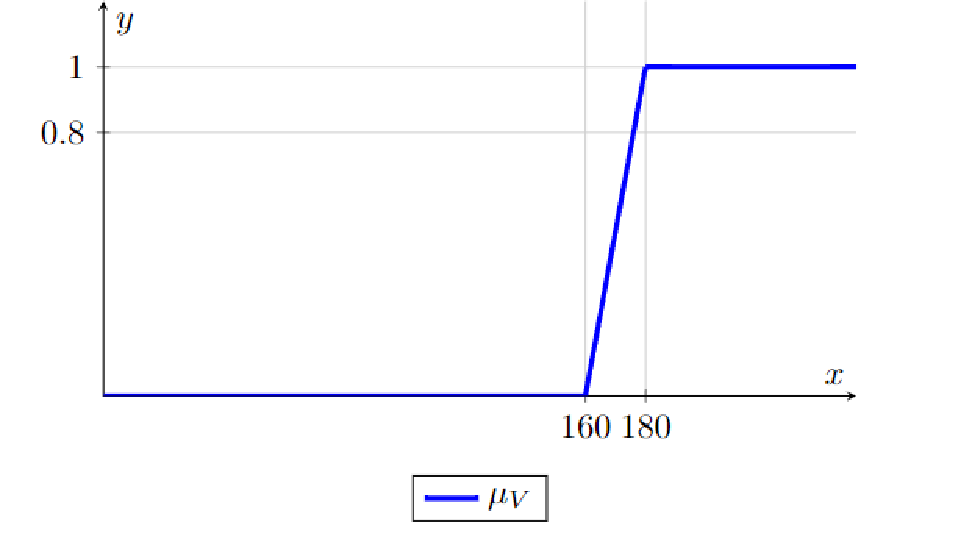
\includegraphics[scale=0.65]{template-fig/vysoky_clovek.pdf}
        \centering
    \end{figure}
\end{graph}     



Pokud bychom chtěli modelovat funkci např. pojmu \clqq asi 3\crqq, lze zvolit několik možných řešení tohoto problému. Každý pak vyjadřuje jiný rozptyl možných řešení.
\begin{graph} Grafické znázornění funkcí příslušnosti výroku P \clqq asi 3\crqq.\\
    \begin{figure}[h]
        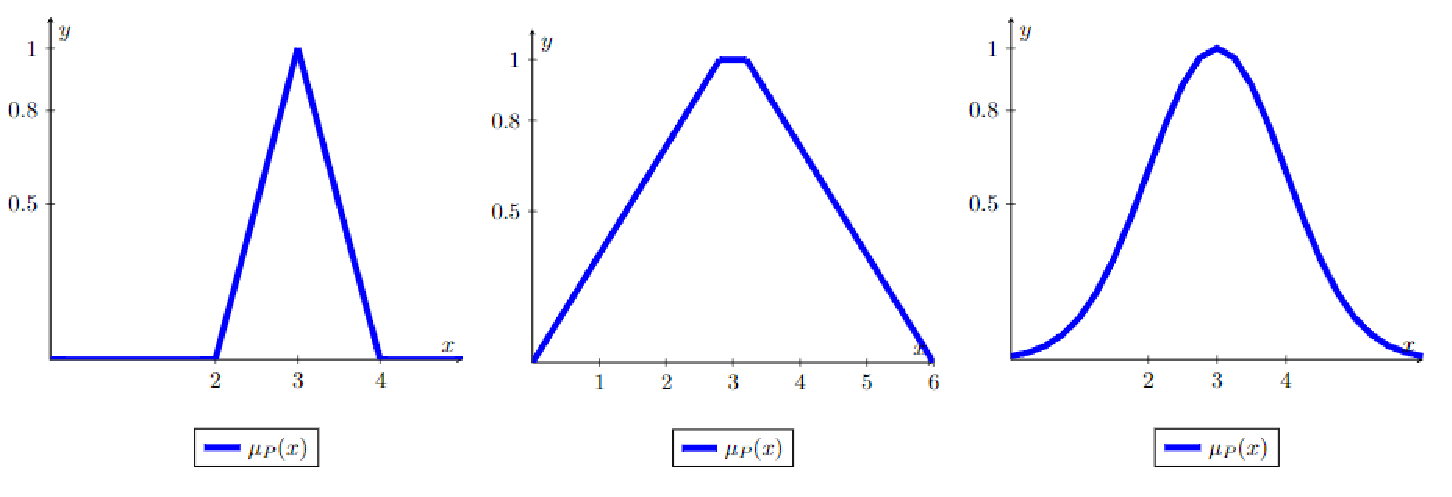
\includegraphics[scale=0.65]{template-fig/asi_3.pdf}
        \centering
    \end{figure}

\end{graph}


\section{Fuzzy logick\'e spojky}

Fuzzy logické spojky n\'am umo\v z\v nují vyjádřit vágnost a neurčitost v logických operacích. Tyto spojky se často využívají v aplikacích jako jsou řízení průmyslových procesů, rozpoznávání vzorů, vývoj umělé inteligence a dalších oblastech, kde je potřeba pracovat s neurčitými informacemi.\\

V\v sechny fuzzy logick\'e spojky jsou monot\'onn\'im roz\v s\'i\v ren\'im klasick\'ych logick\'ych spojek. V dalších kapitolách budou postupně představeny základní fuzzy spojky, mezi kter\'e  patří 
fuzzy negace, konjunkce, disjunkcie a implikace. 

\subsection{Fuzzy negace}

Fuzzy negace představují klíčový koncept v oblasti fuzzy logiky. Tyto negace jsou zobecn\v en\'im klasick\'ych negac\'i. Základní vlastnosti fuzzy negací jsou:

\begin{enumerate}
\item \textbf{Soudržnost:}\\
Pro hodnoty $0$ a $1$ se fuzzy negace shoduje s klasickou negac\'i.
    \item \textbf{Kontinuita hodnot:} \\
        Fuzzy negace nepracuje jenom s  ostrými hodnotami „pravda“ a „nepravda“, ale na stupni neurčitosti, či specifickým číselném zápisu, který reflektuje stupeň nepravdivosti.
    \item \textbf{Monotonie:} \\
        Fuzzy negace jsou monot\'onn\'im roz\v s\'i\v ren\'im klasick\'e negace, což znamená, že s rostoucími vstupn\'imi hodnotami klesaj\'i hodnoty výstupn\'e.
    
\end{enumerate}

\begin{definition}
\cite{Kolo} Fuzzy negací nazýváme každou funkci $N:[0, 1] \to [0, 1]$  s vlastnostmi:
    \begin{enumerate}
        \item  $N(0) = 1, N(1) = 0,$
        \item $\forall  x, y \in [0, 1]: x < y \Rightarrow{} N(x) \geq N(y).$
     \end{enumerate}
\end{definition}
     \begin{example}
         Funkce $N_S(x)=1-x$ spl\v nuje vlastnosti fuzzy negace na intervalu $[0,1].$ Je to nejzn\'am\v ej\v s\'i fuzzy negace, kterou ve sv\'e pr\'aci p\v redstavil Lotfi A. Zadeh a obvykle je ozna\v cov\'ana jako standardn\'i negace.   Fuzzy negace nemus\'i b\'yt nutn\v e spojit\'a funkce. Zn\'am\'e p\v r\'iklady nespojit\'ych fuzzy negac\'i jsou n\'asleduj\'ic\'i funkce:
         $$ N_{\bot}(x)=\begin{cases} 1, & \mbox{pokud }x=0, \\
         0, & \mbox{pokud }x\in \mbox{]0, 1]}, \end{cases} \mbox{  }
         N_{\top}(x)=\begin{cases} 1, & \mbox{pokud }x\in \mbox{[0, 1[}, \\
         0, & \mbox{pokud }x=1. \end{cases}$$
         Funkce $N_{\bot}$ je nejmen\v s\'i a funkce $N_{\top}$ je nejv\v et\v s\'i fuzzy negace, proto
         \begin{equation}
        N_{\bot}(x) \geq N(x) \geq N_\top(x)  \mbox{ pro každé } x \in [0, 1]. \
    \end{equation}
    V literatu\v re jsou negace $N_\bot, N_\top$ zn\'am\'e jako Gödelovy fuzzy negace.
    
    Funkce $N_1(x) = \sqrt{1-x}$ a $N_2(x) = \sqrt{1-x^2}$ jsou zřejmě pro $ x \in [0,1]$ nerostoucí a tak\'e plat\'i:
        \begin{enumerate}
            \item $N_1(0) = \sqrt{1-0} = 1, 
                    N_1(1) = \sqrt{1-1} = 0, $
            \item $N_2(0) = \sqrt{1-0^2} = 1,
                    N_2(1) = \sqrt{1-1^2} = 0.$
        \end{enumerate}
         Tedy i tyto funkce jsou fuzzy negace.

         \begin{graph} Grafy dříve zmíněných funkcí $N_s$, $N_{\bot}$,$ N_{\top}$, $N_1$ a $N_2.$\\
         
            \begin{figure}[h]
                %\hspace{-0.1cm}
                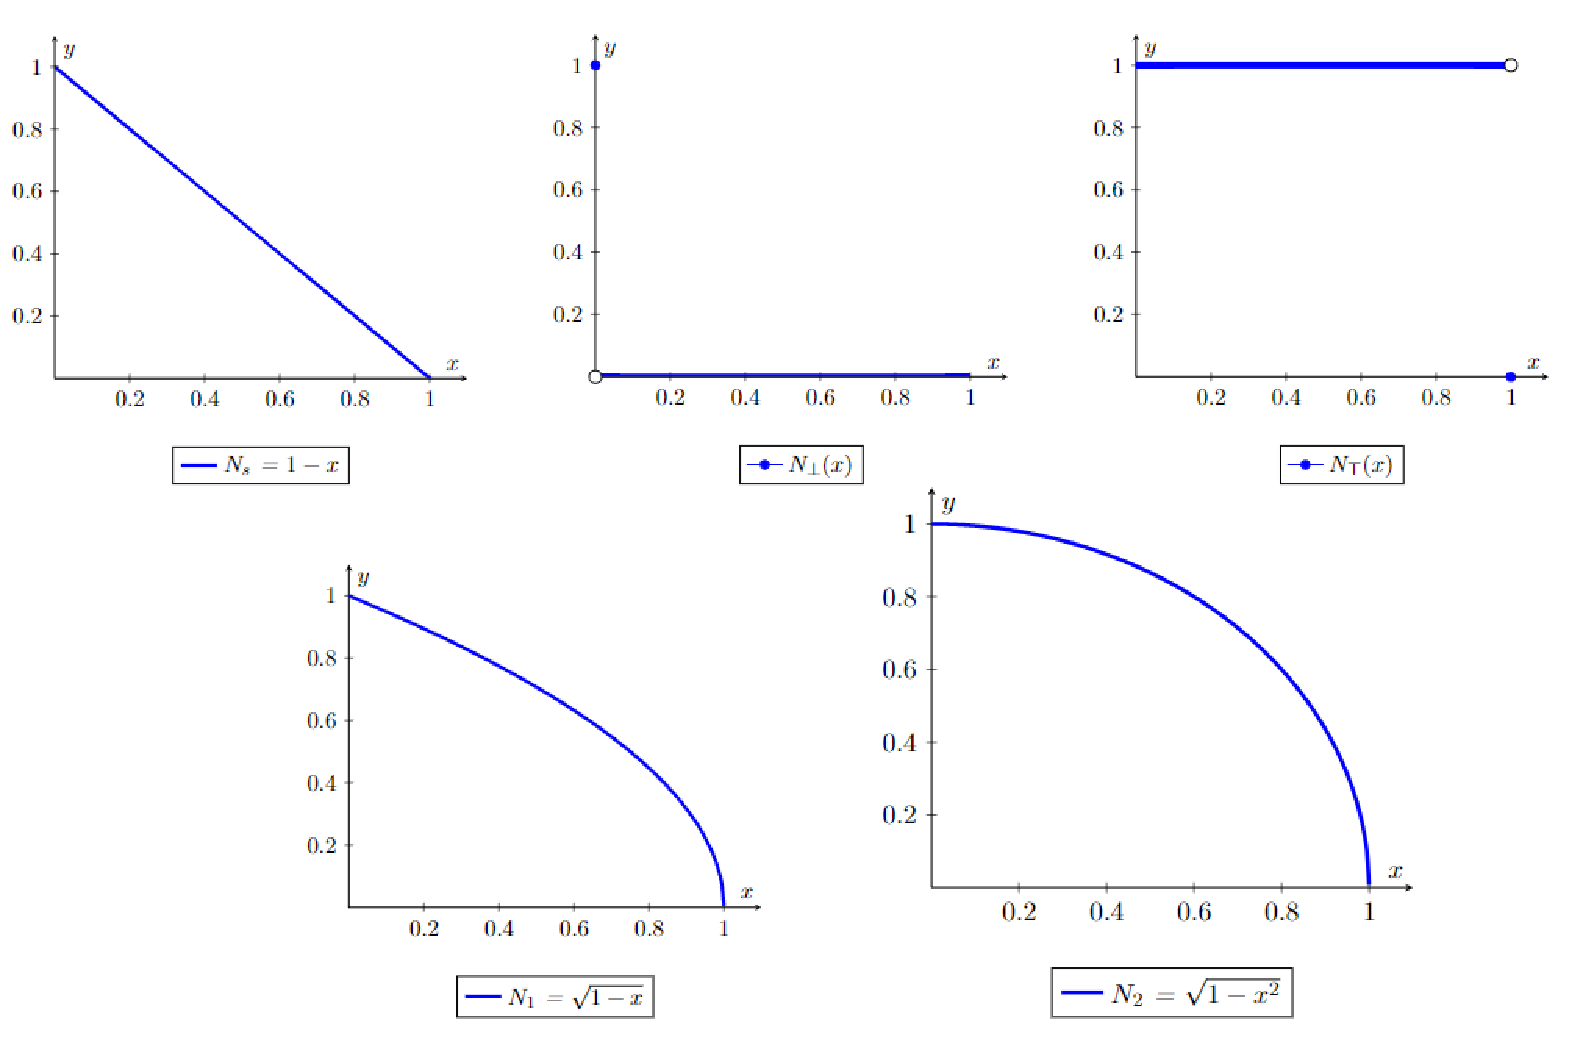
\includegraphics[scale=0.56]{template-fig/negace.pdf}
                \centering
            \end{figure}
        \end{graph}
    \end{example}

   N\v ekter\'e fuzzy negace maj\'i dal\v s\'i zaj\'imav\'e vlastnosti. 

    \begin{definition}
    \cite{Kolo}
        Kdy\v z je $N: [0,1] \to [0,1]$ klesající a spojitá fuzzy negace, nazývá se striktní negace.
        Striktn\'i fuzzy negace, kter\'a je involutivní, tedy, pro kterou plat\'i $N(N(x)) = x $ pro každé $ x \in [0,1]$, se nazývá silná fuzzy negace.
    \end{definition}

    \begin{example}
        Spojit\'e neg\'atory $N_S, N_1, N_2$ z p\v redchoz\'iho p\v rikladu jsou evidetn\v e striktn\'i, proto\v ze jsou ryze monot\'onn\'i. D\'ale plat\'i:
        $$N_S(N_S(x))=1-(1-x)=x, \mbox{pro ka\v zd\'e } x \in [0,1],$$
                $$N_1(N_1)) = N_1(\sqrt{1-x}) = \sqrt{1-\sqrt{1-x}} \neq x, \mbox{ pro t\'em\v e\v r každé } x \in ]0,1[,$$ $$N_2(N_2) = N_2(\sqrt{1-x^2}) = \sqrt{1-(\sqrt{1-x^2})^2} = x,
                \mbox{pro každé } x \in [0,1].$$
Takže negace $N_S$ a $N_2$ jsou involutivní a tím pádem tak\'e siln\'e negace, naopak
            negace $N_1$ není involutivní, tedy ani siln\'a fuzzy negace.
                
            \end{example}

    \begin{remark}
        Z rovnosti $N(N(x))=x$ plyne pro bijektivn\'i funkce tak\'e rovnost $N(x)= N^{-1}(x).$ 
         Grafick\'a interpretace  t\'eto rovnosti  pro fuzzy negace je taková, že grafy involutivních fuzzy negací jsou osově souměrné podle osy $y = x$.
        \begin{graph} Ukázka osové souměrnosti bijektivní funkce f(x) = $\sqrt{1-x^2}$ podle osy y = x pro $x \in [0,1]$.\\
            
            \begin{figure}[h]
                \hspace{-1cm}
                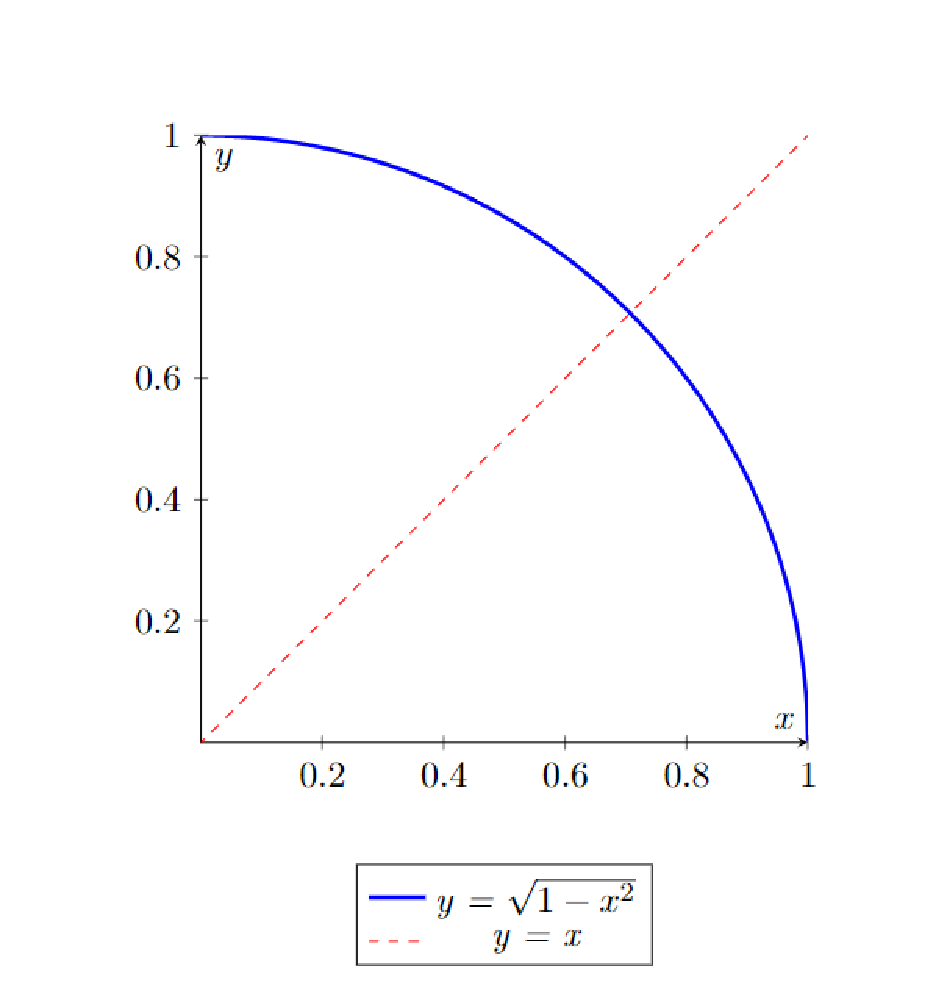
\includegraphics[scale=0.65]{template-fig/soumernost.pdf}
                \centering
            \end{figure}
        \end{graph}
    \end{remark}


    
\subsection{Fuzzy konjunkce}

Fuzzy konkjunkce se využívají pro spojení dvou a více podmínek s ohledem na jejich vágnost a neostrost. Místo výsledného \clqq ano\crqq \space nebo \clqq ne\crqq \space je použita hodnota  $x \in [0,1]$, která reprezentuje, do jaké míry jsou podmínky splněny.  
Základní vlastnosti fuzzy konjunkcí jsou:
\begin{enumerate}
    \item \textbf{Soudržnost:}\\
    Pro hodnoty 0 a 1 se fuzzy konjunkce shoduje s klasickou konjunkcí.
    \item \textbf{Kontinuita hodnot:}\\
    Fuzzy konjunkce nepracuje jenom s  ostrými hodnotami „pravda“ a „nepravda“, ale na stupni neurčitosti či specifickým číselném zápisu, který reflektuje stupeň pravdivosti.
    \item \textbf{Monotonie:}\\
    Fuzzy konjunkce je monot\'onní operace, což znamená, že s rostoucími vstupními hodnotami rostou i výsledky jejich konjunkce.
\end{enumerate}
\begin{definition}
    \cite{KMP}
    Neklesající zobrazení C: $[0,1]^2 \rightarrow [0,1]$ se nazývá konjunktor, pokud pro libovolné a,b $\in$ [0,1] platí
    C(a,b) = 0 pokud a = 0, nebo b = 0,
    C(1,1) = 1.
    \end{definition}

\begin{remark}
    Fuzzy konjunkce mohou být modelovány pomocí triangulárních norem, kterým je věnována celá následující podkapitola.
\end{remark}

\subsection{Triangul\'arn\'i normy} 

Jak již bylo zmíněno, fuzzy konjunkce mohou být modelov\' any pomocí triangulárních norem, zjednodušeně t-norem. 
\begin{definition}
\cite{KMP}
    Triangulární norma je binární operace na jednotkovém intervalu [0,1], t.j. funkce $T: [0,1]^2 \rightarrow [0,1]$ taková, že pro každé $x, y, z \in [0,1]$ jsou splněné následující axiomy:
    \begin{enumerate}
        \item \textbf{Komutativnost:} $T(x,y) = T(y,x)$,
        \item \textbf{Asociativita:} $T(x, T(y, z)) = T(T(x, y), z)$,
        \item \textbf{Monotónnost:} pokud $y \geq z$ pak $T(x, y) \geq T(x, z)$,
        \item \textbf{Okrajová podmínka:} $T(x, 1) = x$.
    \end{enumerate}
\end{definition}

\begin{example} N\'asleduj\'ic\'i funkce vždy spl\v nují 3 ze 4  axiom\r u, což ukazuje, že jsou na sobě axiomy nez\' avislé, a tedy funkce není t-normou, pokud nespl\v nuje všechny čtyři axiomy.\\ 
    Funkce $F_1 : [0, 1]^2 \to [0, 1]$ daná přepisem
    $$F_1(x,y) = x,$$
    spl\v nuje axiomy 2., 3., 4., ale nespl\v nuje axiom 1.
    
    Funkce $F_2 : [0, 1]^2 \to [0, 1]$ daná přepisem
    $$F_2(x,y) = x.y.\max(x,y),$$
    spl\v nuje axiomy 1., 3., 4., ale nespl\v nuje axiom 2.

    Funkce $F_3 : [0, 1]^2 \to [0, 1]$ daná přepisem
    $$ F_3(x,y)=\begin{cases} 0.5, & \mbox{pokud }(x, y) \in ]0,1[^2, \\
         \min(x,y), & \mbox{jinak,}\end{cases} $$
    spl\v nuje axiomy 1., 2., 4., ale nespl\v nuje axiom 3.
    
    Funkce $F_4 : [0, 1]^2 \to [0, 1]$ daná přepisem
    $$F_4(x,y) = 1,$$
    spl\v nuje axiomy 1., 2., 3., ale nespl\v nuje axiom 4.

  \end{example}

Mezi základní triangulární normy se řadí minimová, součinová, Łukasiewiczova t-norma a drastický součin.
\begin{example}
\cite{KMP}
    \begin{enumerate}
    \item \textbf{Minimová t-norma} $T_M: [0,1]^2 \rightarrow [0,1]$
    $$T_M(x,y) = \min(x,y).$$
    \item \textbf{Součinová t-norma} $T_P: [0,1]^2 \rightarrow [0,1]$
    $$T_P(x,y) = x.y.$$
    \item \textbf{Łukasiewiczova t-norma} $T_L: [0,1]^2 \rightarrow [0,1]$
    $$T_L(x,y) = \max(x+y-1,0).$$
    \item \textbf{Drastický součin} $T_D: [0,1]^2 \rightarrow [0,1]$
    $$T_D:(x)=\begin{cases} \min(x,y), & \mbox{pokud }  \max(x,y) = 1,\\ 
    0, &  jinak.  \end{cases}$$\\
\end{enumerate}
\end{example}


\begin{graph} Minimová t-norma $T_M$, Součinová t-norma $T_P$, Łukasiewiczova t-norma $T_L$, Drastický součin $T_D$.
   \begin{figure}[H]
    \hspace{-1cm}
        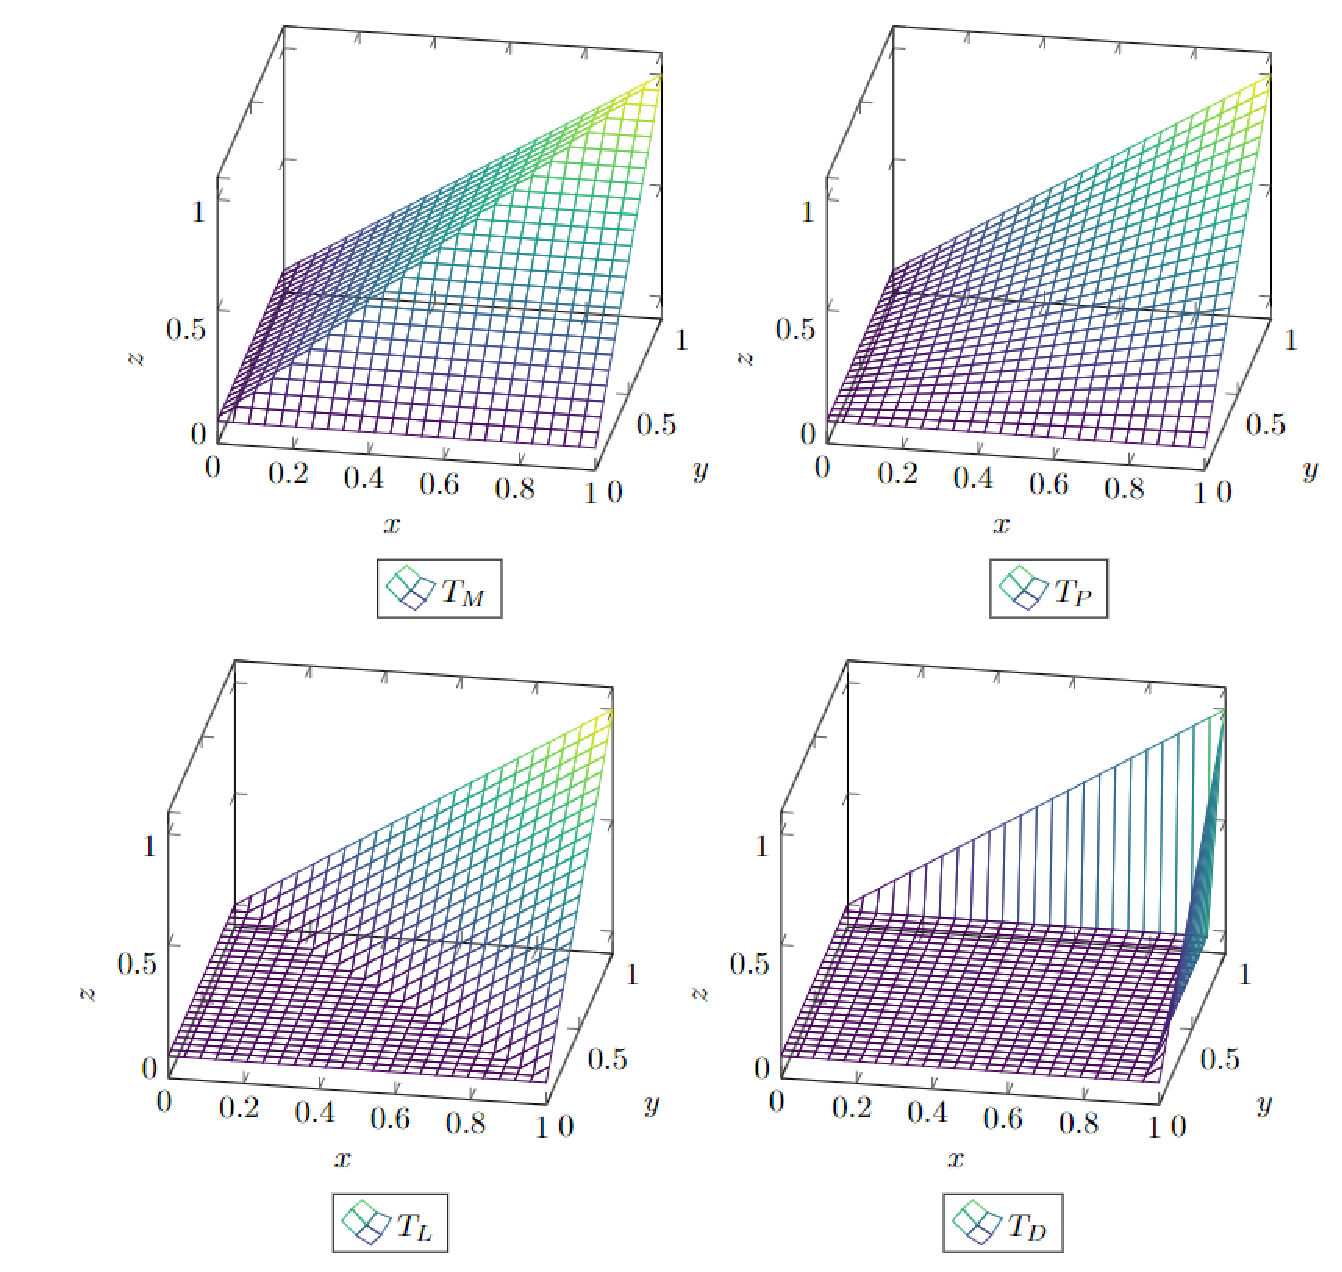
\includegraphics[scale=0.7]{template-fig/t_normy.pdf}
        \centering
    \end{figure}
\end{graph}

\begin{remark}
    Je zřejmé, že pro každou t-normu T platí
    $$T(1,x)=T(x,1)=x,$$
    $$T(0,x)=T(x,0)=0.$$
\end{remark}
\begin{definition}
\cite{KMP}
    \begin{itemize}
        \item Pokud pro t-normy $T_1$ a $T_2$ je
        pro každý bod $(x,y) \in [0,1]^2$ splněná nerovnost\\
        $T_1(x,y)\leq ~T_2(x,y),$ hovo\v ríme, že $T_1$ je slabší než $T_2$,
        nebo $T_2$ je silnější než $T_1$ a píšeme $T_1\leq T_2$.
        \item  Pokud pro t-normy $T_1$ a $T_2$ platí, že $T_1 \leq T_2$ a
        $T_1 \ne T_2,$ t.j. pokud $T_1 \leq T_2$, ale $T_1(x_0,y_0) <
        T_2(x_0,y_0)$ pro nějaký bod $(x_0,y_0) \in [0,1]^2$, tak $T_1<T_2$.
    \end{itemize}
\end{definition}


Existuje nekone\v cn\v e mnoho t-norem, dokonce pak i cel\'e t\v r\'idy parametrick\' ych  t-norem. Mezi nejzn\' am\v ej\v s\' i parametrické třídy patří:
\begin{itemize}
    \item \textbf{Frankovy t-normy:}
    $$T_p^F:(x,y)=\begin{cases} T_M(x,y), & \mbox{pokud }  p = 0,\\ 
                                T_P(x,y), & \mbox{pokud } p = 1,\\
                                T_L(x,y), & \mbox{pokud } p = +\infty,\\
                                \log_p(1+\frac{(p^x-1)(p^y-1)}{p-1}), & \mbox{pokud } jinak, 
                                \end{cases}$$
    \item \textbf{Schwarz-Skalarovy t-normy:}
    $$T_p^{SS}:(x,y)=\begin{cases} T_M(x,y), & \mbox{pokud }  p = -\infty,\\ 
                                (x^p+y^p-1)^\frac{1}{p}, & \mbox{pokud }  -\infty < p < 0,\\ 
                                T_P(x.y), & \mbox{pokud } p = 0,\\
                                T_D(x,y), & \mbox{pokud } p = +\infty,\\
                                (\max(0, x^p+y^p-1))^\frac{1}{p}, & \mbox{pokud } 0 < p < +\infty, \end{cases}$$
    \item \textbf{Yagerovy t-normy:}
    $$T_p^Y:(x,y)=\begin{cases}  T_D(x,y), & \mbox{pokud } p = 0,\\
                                \max(0,1-((1-x)^p+(1-y)^p)^\frac{1}{p} , & \mbox{pokud } 0 < p < +\infty,\\
                                T_M(x,y), & \mbox{pokud } p = +\infty,
                                \end{cases}$$
    \item \textbf{Sugeno-Weberovy t-normy:}
    $$T_p^{SW}:(x,y)=\begin{cases}  T_D(x,y), & \mbox{pokud } p = -1,\\
                                    \max(0,\frac{x+y-1+pxy}{1+p}) , & \mbox{pokud } -1 < p < +\infty,\\
                                    T_P(x,y), & \mbox{pokud } p = +\infty.
                                    \end{cases}$$
\end{itemize}

\subsection{Algebraick\'e vlastnosti t-norem}

Každou \' usečku délky $b$ lze pokrýt nějakým počtem \' useček délky $a > 0.$ Tato věta lze vyjádřit i jinak: pro dvě libovolná kladná a reálná čísla $a,b$ existuje přirozené číslo $n$ takové, že $a\cdot n>b,$ což je archimedovská vlastnost reálné osy vzhledem ke sčítání. Velmi podobně je definována i archimedovská vlastnost pro násobení. Pro t-normy je pak archimedovská vlastnost definována následovně:
\begin{definition}
\cite{KMP}
    T-norma je archimedovská, pokud pro všechny body $(x,y) \in ]0,1[^2$ existuje $n \in N$ takové, že $$x_T^{(n)} < y,$$
    p\v ri\v cem\v z $x^{(n)}_T=\begin{cases} x, &\mbox {pokud $n=1,$} \\ {T(x,x_T^{(n-1)})},
&\mbox {pokud $n>1.$}\end{cases}$

\end{definition}
Ověřit archimedovskou vlastnost lze následovným zp\r usobem:
\begin{sentence} \cite{KMP}
    Triangulární norma T je archimedovská právě, když pro každé $(x,y) \in ]0,1[^2$ je $$\lim_{n \to \infty}x_T^{(n)} = 0.$$
\end{sentence}
\begin{sentence} \cite{KMP}
    Pokud je t-norma T archimedovská, tak pro každé $x \in ]0,1[$ platí $T(x,x) < x.$\\
    Pokud je t-norma spojitá zprava, pak je archimedovská právě, když pro každé $x \in ]0,1[$ platí $T(x,x) < x.$
\end{sentence}

    Díky p\v redchozí v\v et\v e lze  archimedovskou vlastnost t-norem pro zprava spojit\'e t-normy také definovat pomocí diagonální nerovnosti $$T(x,x) < x, \mbox{ pro } x \in ]0,1[.$$

    Nejd\r uležitější algebraickou vlastností funkcí je monot\' onnost. U t-norem se pak rozlišuje několik r\r uzných typ\r u monot\' onnosti:
    \begin{definition}
    \cite{KMP}\\
        \begin{itemize}
            \item T-norma $T$ je {\em striktně
            monot\' onní}, pokud
            je rostoucí na $]0,1]^2$ jak funkce $ T:[0,1]^2 \rightarrow [0,1]$ anebo
            ekvivalentně,
            $$ \text {pokud} \hskip 3mm x \in \hskip 1mm ]0,1] \hskip 3mm \text{a} \hskip 3mm y < z, \hskip 3mm \text {tak} \hskip 3mm T(x,y) < T(x,z). $$
            \item  T-norma $T$ je {\em sdruženě striktně
            monot\' onní}, pokud platí:
            $$ \text{pokud} \hskip 3mm  x < x'\hskip 3mm \text{a} \hskip 3mm y<y',
            \hskip 3mm  \text{tak} \hskip 3mm   T(x,y)<T(x',y').$$
            \end{itemize}
    \end{definition}

    Dal\v s\'i d\r uležité  pojmy jsou \textit{dělitel nuly a nilpotentn\'i prvek}:
    \begin{definition}
        \cite{KMP}\\
        Prvek $x \in ]0,1[$ lze nazvat {\em dělitelem nuly} dané t-normy $T$, pokud
        existuje $y \in ]0,1[$ takové, že $T(x,y) = 0.$
        Prvek $x \in ]0,1[$ je {\em nilpotentním prvkem dané t-normy $T$}, pokud existuje $n \in N$ takové,
        že $ x_T^{(n)} =0.$
    \end{definition}

    \begin{example}
        Je zřejmé, že výše zmíněné t-normy $T_P$ a $T_M$ nemají ani nilpotentní prvek, ani dělitele nuly. Naopak pro t-normy $T_D$ a $T_L$ platí, že každé $x \in ]0,1[$ je dělitelem nuly a i nilpotentním prvkem těchto t-norem.
    \end{example}

    \begin{definition}
    \cite{KMP}
        Triangul\'arn\'i norma $T$ se naz\'yv\'a {\em nilpotentní}, pokud je spojitá a každé $x
        \in ]0,1[$ je jejím nilpotentním prvkem.
    \end{definition}    
    \begin{definition}
    \cite{KMP}
        Triangul\'arn\'i norma $T$ se naz\'yv\'a {\em striktní}, pokud je
            spojitá a striktně monot\' onní.
    \end{definition} 
    
     Vztah nilpotentních a striktních t-norem, které jsou archimedovské a spojité, lze pak vyjádřit následovně:
    \begin{sentence}\cite{KMP}
        Nech\' t je T spojitá archimedovská t-norma. Potom jsou následující tvrzení ekvivalentní:
        \begin{itemize}
        \item T je nilpotentní.
        \item  Existuje alespo\v n jeden nilpotentní prvek dané t-normy T.
        \item T není striktní.
        \item  T má dělitele nuly.
        \end{itemize}
    \end{sentence}
    Mezi nejtypičtější příklady nilpotentních t-norem patří Łukasiewiczova t-norma a všechny archimedovsk\'e, nilpotentní t-normy jsou s ní izomorfní. Naopak, v\v sechny archimedovsk\'e, striktn\'i t-normy jsou izomorfn\'i se sou\v cinovou t-normou $T_P.$
    

\subsection{Konstrukce triangulárních norem}

V t\'eto pr\'aci se v\v enuji tak\'e konstrukc\'im t-norem. Triangul\'arn\'i normy lze konstruovat pomoc\'i funkc\'i jedn\'e prom\v enn\'e, ale tak\'e z ji\v z existuj\'ic\'ich t-norem. Mezi nejznámější konstrukce t-norem patří:
\begin{itemize}
    \item \textbf{Ordinální součet:}
    \cite{KMP}
        Nech\v t $(T_\alpha)_{\alpha \in A}$ je třída t-norem a
        nech\v t $(]a_\alpha,e_\alpha[)_{\alpha \in A}$ je třída po dvojcích
        disjunktních otevřených podinterval\r u intervalu $[0,1].$ Potom funkce
        \hbox{$T:[0,1]^2\rightarrow [0,1]$} daná předpisem
        $$T(x,y)=\begin{cases} a_\alpha + (e_\alpha - a_\alpha ).T_\alpha (\frac
        {x-a_\alpha}{e_\alpha - a_\alpha}, \frac {y-a_\alpha}{e_\alpha - a_\alpha}),
        &\mbox {pokud $(x,y) \in ]a_\alpha ,e_\alpha [^2$,}
        \\\min(x,y), &\mbox {jinak,} \end{cases}$$
        je t-normou, kterou nazývame {\em ordinálním součtem} sčítanc\r u $\langle a_\alpha ,e_\alpha
        ,T_\alpha \rangle,$ \mbox{$ \alpha \in A.$}

    \item \textbf{Aditivní a multiplikativní generování:}
        \cite{KMP}
        Nech\v t je funkce $f:[0,1] \to [0,\infty]$ spojitá a klesající, přičemž
        $f(1)=0$, potom je předpisem
        $$ T_{<f>}(x,y)=f^{-1}(\min(f(x)+f(y),f(0)))$$
        dána t-norma a funkce $f$ se nazývá aditivní generátor t-normy
        $T_{<f>}.$
        
        Nech\v t je funkce $g:[0,1] \to [0,1]$ spojitá a rostoucí, přičemž
        $g(1)=1$, potom je předpisem
        $$ T^{<g>}(x,y)=g^{-1}(\max(g(x).g(y),g(0)))$$
        dána t-norma a funkce $g$ se nazývá multiplikativní generátor t-normy
        $T^{<g>}.$
    \item \textbf{$\varphi$-transformace}
        \cite{KMP}
        Pokud je $\varphi$ rostoucí bijekce uzavřeného jednotkového intervalu, potom
        předpisem
        $$T_\varphi (x,y)=\varphi ^{-1}(T(\varphi(x),\varphi(y)))\space \text {pro $(x,y)
        \in [0,1]$}$$
        je dána t-norma, kterou nazýváme $\varphi-${\em transformací t-normy}
        $T.$

\end{itemize}

\begin{remark}
    Triangul\'arn\'i norma $T$ je striktní právě tehdy, když pro její aditivní generátor platí $f(0) = +\infty$. Nilpotentní je v momentě, když pro  její aditivní generátor platí $f(0) < +\infty$.
\end{remark}
\subsection{Pseudoinverzn\'i funkce}

Krom\v e   spojit\'ych t-norem existuj\'i tak\'e t-normy nespojit\'e a dokonce se daj\'i generovat. Jak je tedy možné konstruovat nespojité t-normy? Například funkce $t: [0,1] \rightarrow [1,2],$ daná předpisem $$t(x)= \begin{cases} 2-x, & \mbox {pokud }x \in [0,1[,
    \\ 0, & \mbox {pokud} x = 1,
    \end{cases}$$
    
    je aditivním generátorem drastického součinu, což zřejmě znamená, že generátory nespojitých t-norem nemusejí být nutně bijekce. Z toho d\r uvodu je potřeba zobecnění inverzní funkce.

      Pro neklesající  funkce je definice zobecn\v en\'e inverzn\'i funkce n\'asledovn\'i:
\begin{definition}
    \cite{hlinena}
    Nech\v t je $f:[a,b] \rightarrow [c,d]$ neklesající funkce, pak pro každé $y \in [c,d]$ je předpisem $$f^{(-1)}(y) = sup(x \in [a,b];f(x)<y)$$
    definována pseudoinverzní funkce $f^{(-1)}$ k dané funkci f.
\end{definition}

Pro lep\v s\'i pochopen\'i t\'eto definice, uv\'ad\'ime ilustra\v cn\'i p\v r\'iklady:

\begin{example} 
    Nech\v t je  $f_1:[0,1] \rightarrow [0,1]$  dána předpisem:
    $$f_1(x)=x^2.$$
   Pro bijektivn\'i funkce jsou inverzn\'i a pseudoinverzn\'i funkce toto\v zn\'e: \newline$f_1^{(-1)}:[0,1] \rightarrow [0,1]$ zřejmě bude platit:
    $$f_1^{(-1)}(x)=f_1^{-1}(x)= \sqrt{x}.$$
    Proto složením funkcí $f_1$ a $f_1^{(-1)}$ je
    identita na intervale $[0,1].$
\end{example} 

    \begin{graph} Ukázka složení funkcí $f_1^{(-1)} $ a $ f_1$, nebo také zevšeobecnění inverzní funkce.\\

   \begin{figure}[H]
                \hspace{-1cm}
                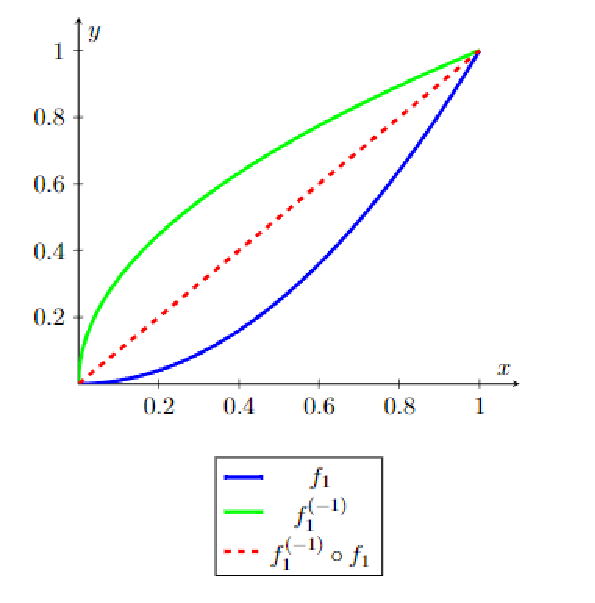
\includegraphics[scale=0.75]{template-fig/inverz.pdf}
                \centering
            \end{figure}
\end{graph}


\begin{example}
\label{sec: funkce}
\cite{hlinena}
\begin{enumerate}
    \item Nech\v t je $f_2:[0,1] \rightarrow [0,1]$ dána předpisem:
    $$f_2(x)= \begin{cases} \frac x2, & \mbox{pokud~} x \in [0,\frac 12],
    \\ \frac 14, & \mbox{pokud~} x \in ]\frac 12,\frac 34],
    \\ 3.x-2, & \mbox{pokud~} x \in ]\frac 34,1].
    \end{cases}$$
    Funkce $f_2$ není injekce, což znamená, že k ní neexistuje inverzní funkce. Na intervalu $[0,\frac 12]$ je funkce $f_2$ spojitá a injektivní, proto na daném oboru hodnot $[f(0),f(\frac 12)]$ je
    funkce $f_2^{(-1)}$ totožná s~inverzní funkcí
    $f_{2/[f(0),f(\frac 12)]}^{-1}.$
    Potom pro monot\'onní rozšíření inverzní funkce plat\'i
    $$f_2^{(-1)}(x)= \begin{cases} 2x, & \mbox {pokud $x \in [0,\frac 14],$}
    \\ \frac x3 + \frac 23, & \mbox {pokud $x \in ]\frac 14,1].$}
    \end{cases}$$
    Složení funkcí pak bude vypadat následovně:
    $$g(x)=f_2^{(-1)} \circ f_2(x)=f_2^{(-1)} \left(f_2(x)\right)= \begin{cases} \frac 12,
    & \mbox{pokud $x \in [\frac 12,\frac 34],$}
    \\x, & \mbox {jinak.} \end{cases}$$
    
    \item Nech\v t je $f_3:[0,1] \rightarrow [0,1]$ dána předpisem:
    $$f_3(x)= \begin{cases} 2x, & \mbox {pokud $x \in [0,\frac 14],$}
    \\ \frac x3 + \frac 23, & \mbox {pokud $x \in ]\frac 14,1].$}
    \end{cases}$$
    Funkce $f_3$ je injektivní, takže k ní narozdíl od funkce $f_2$ existuje inverzní funkce. Jenomže funkce $f_3$ není bijektivní, tudíž její inverzní funkce nebude definována na celém intervalu $[0,1]$. 
    Její jediné monot\' onní rozšíření na celý interval $[0,1]$ je dáno předpisem
    $$f_3^{(-1)}(x)= \begin{cases} \frac x2, & \mbox {pokud $x \in [0,\frac 12],$}
    \\ \frac 14, & \mbox {pokud $x \in ]\frac 12,\frac 34],$}
    \\ 3.x-2, & \mbox {pokud $x \in ]\frac 34,1]$.}
    \end{cases}$$
\end{enumerate}
\end{example}
Následující grafy zobrazují zmíněné funkce $f_2$ a $f_3$ a jejich složení s inverzními funkcemi.\\

\begin{graph} Zobrazení funkcí z Příkladu \ref{sec: funkce}. Modře jsou vyznačeny (zleva) funkce $f_2$ a $f_3$, zeleně jejich zevšeobecněné inverzní funkce a červeně složené funkce $f_2^{(-1)} \circ f_2(x) $~a~$ f_3^{(-1)}\circ ~f_3(x).$
\label{sec: inverz}
     \begin{figure}[H]
                \hspace{-1cm}
                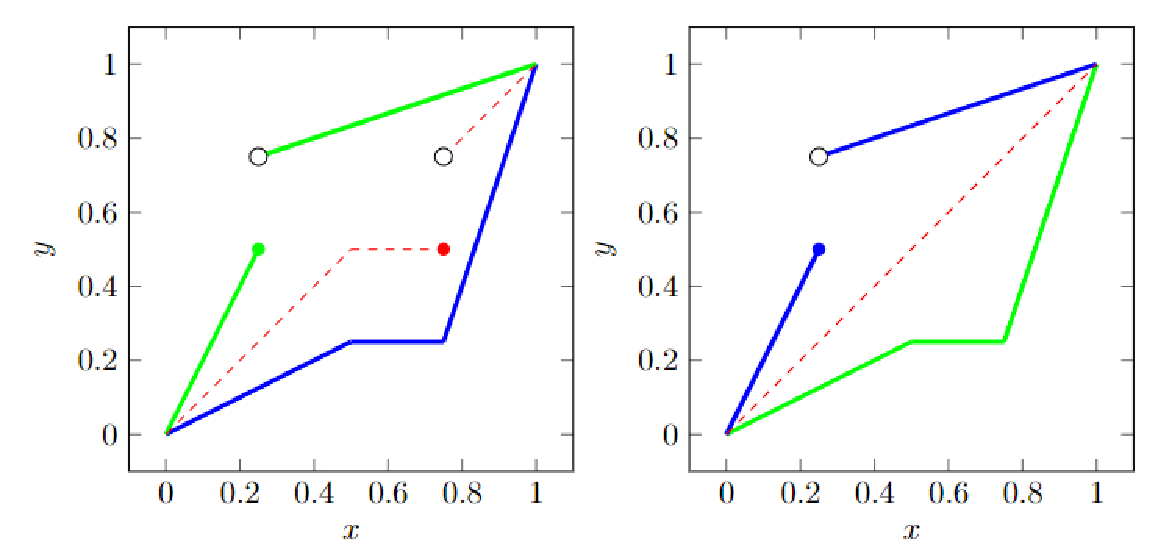
\includegraphics[scale=0.65]{template-fig/zevs_inverz.pdf}
                \centering
            \end{figure}

            
\end{graph}

Na Obrázku \ref{sec: inverz} lze zřejmě pozorovat následující situaci: $$f_2(x)=f_3^{(-1)}\text{ a } f_3(x)=f_2^{(-1)}(x), \text{ takže } (f_2^{(-1)})^{(-1)}(x)=f_2(x) \text{ a }
            (f_3^{(-1)})^{(-1)}(x)=f_3(x).$$ 
            
 Pro nerostouc\'i funkce je definice a tak\'e konstrukce pseudoinverzn\'i funkce analogick\'a: 
\begin{definition}
    \cite{hlinena}
    Nech\v t je $f:[a,b] \rightarrow [c,d]$ nerostoucí (nekonstantní) funkce, pak pro každé $y \in [c,d]$ je předpisem $$f^{-1}(y) = sup(x \in [a,b];f(x)>y)$$
    definována pseudoinverzní funkce $f^{(-1)}$ k dané funkci f.
\end{definition}


\begin{remark} Na předchozích příkladech bylo naznačeno konstruování pseudoinverzní funkce. Nech\v t je $f:[a,b] \rightarrow [x,d]$ neklesající funkce, lze si pak všimnout určitých poznatk\r u:
    \begin{itemize}
        \item pokud je funkce $f$ bijekce, tak platí $f^{(-1)}(x) = f^{-1}(x),$
        \item  pokud je funkce $f$ rostoucí, její pseudoinverzní funkce je spojitá,
        \item  pro každé $x \in [a,b]$ platí: $f^{(-1)}\circ f(x)\leq x.$
    \end{itemize}
    Nech\v t je $f:[a,b] \rightarrow [x,d]$ nerostoucí funkce:
    \begin{itemize}
        \item pokud je funkce $f$ bijekce, tak platí $f^{(-1)}(x) = f^{-1}(x),$
        \item  pokud je funkce $f$ klesající, její pseudoinverzní funkce je spojitá,
        \item  pro každé $x \in [a,b]$ platí: $f^{(-1)}\circ f(x)\leq x.$
    \end{itemize}
\end{remark}

 Zobecn\v en\'i inverzn\'i funkce n\'am d\'av\'a mo\v znost zobecnit aditivn\'i i multiplikativn\'i generov\'an\'i t-norem:
\begin{sentence} \cite{KMP}
    Nech\v t je $f:[0,1] \rightarrow [0,\infty]$ klesající funkce
    taková, že $f(1)=0$ a pro všechny $(x,y) \in [0,1]^2$  je splněno
    $$f(x)+f(y) \in H(f) \cup [f(0)^+,\infty].$$
    Potom funkce dvou proměnných $T:[0,1]^2 \rightarrow [0,1]$ dána předpisem
    $$T(x,y)=f^{(-1)}(f(x)+f(y))$$
    je triangulární norma.
\end{sentence}
\begin{sentence}\cite{KMP}
    Nech\v t je $l:[0,1] \rightarrow [0,1]$ rostoucí funkce
    taková, že $l(1)=1$ a pro všechny $(x,y) \in [0,1]^2$  je splněno
    $$l(x).l(y) \in H(l) \cup [0,l(0)^+].$$
    Potom funkce dvou proměnných $T:[0,1]^2 \rightarrow [0,1],$ dána předpisem
    $$T(x,y)=l^{(-1)}(l(x).l(y)),$$
    je triangulární norma.
\end{sentence}


\subsection{Fuzzy disjunkce} 
Fuzzy disjunkce vyjadřuje, stejně jako fuzzy konjunkce, míru spojení dvou či více prvk\r u. Výsledek fuzzy disjunkce je hodnota $x \in [0,1].$ 
Základní vlastnosti fuzzy disjunkcí jsou:
\begin{enumerate}
    \item \textbf{Soudržnost:}\\
    Pro hodnoty 0 a 1 se fuzzy disjunkce shoduje s klasickou disjunkcí.
    \item \textbf{Kontinuita hodnot:}\\
    Fuzzy disjunkce nepracuje jenom s  ostrými hodnotami „pravda“ a „nepravda“, ale na stupni neurčitosti či specifickým číselném zápisu, který reflektuje stupeň spojení prvk\r u.
   \item \textbf{Monotonie:}\\
    Fuzzy disjunkce je monotonní operace, což znamená, že s klesajícími vstupními hodnotami klesají i výsledky jejich disjunkce.
\end{enumerate}

\begin{definition}
    \cite{Kolo}
    Neklesající zobrazení $D: [0,1]^2 \rightarrow [0,1]$ se nazývá disjunktor, pokud pro libovolné $a, b \in [0,1]$ platí\\ $D(a,b) = 1$ pokud  $a = 1$, nebo  $b = 1,$\\
    $D(0,0) = 0.$
\end{definition}

Nej\v cast\v eji pou\v z\'iv\'any funkce pro modelov\'an\'i fuzzy disjunkce jsou triangul\'arn\'i konormy, kter\'ym je v\v enov\'ana n\'asleduj\'ic\'i podkapitola.

\subsection{Triangul\'arn\'i konormy} 
\label{sec: Triangulární konormy}

Triangulární konormy (zkráceně t-konormy) jsou, podobn\v e jako  t-normy, re\'aln\'e funkce dvou prom\v enn\'ych:
\begin{definition}
    Triangulární konorma je binární operace na intervalu $[0,1],$ t.j. funkce $S: [0,1]^2 \rightarrow [0,1]$ taková, že pro každé $x, y, z \in [0,1]$ jsou splněny následující axiomy:
    \begin{enumerate}
        \item \textbf{Komutativnost: } $S(x,y) = S(y,x),$
        \item \textbf{Asociativita: } $S(x,S(y,z)) = S(S(x,y),z)$,
        \item \textbf{Monotónnost:} pokud $y \leq z$ pak $S(x, y) \leq S(x, z)$,
        \item \textbf{Okrajová podmínka: } $S(x,0) = x.$
    \end{enumerate}
\end{definition}

Triangulární konormy (zkráceně t-konormy) a t-normy jsou du\'aln\'i funkce:

\begin{sentence}
    \cite{Springer}
    Pokud je $T:[0,1]^2\to [0,1]$ t-norma, tak její duální t-konorma $S: [0,1]^2 \rightarrow [0,1]$ je dána předpisem $$S(x,y) = 1 - T(1-x, 1-y).$$
\end{sentence}


Mezi základní triangulární konormy se obdobně (ale komplementárně) jako u t-norem řadí maximová a Łukasiewiczova t-norma, pravděpodobnostní a drastický součet.
\begin{example}
\cite{Springer}
    \begin{enumerate}
    \item \textbf{Maximová t-konorma} $S_M: [0,1]^2 \rightarrow [0,1]$
    $$S_M(x,y) = \max(x,y).$$
    \item \textbf{Pravděpodobnostní součet} $S_P: [0,1]^2 \rightarrow [0,1]$
    $$S_P(x,y) = x+y-x.y.$$
    \item \textbf{Łukasiewiczova t-konorma} $S_L: [0,1]^2 \rightarrow [0,1]$
    $$S_L(x,y) = \min(x+y,1).$$
    \item \textbf{Drastický součet} $S_D: [0,1]^2 \rightarrow [0,1]$
    $$S_D:(x)=\begin{cases} \max(x,y), & \mbox{pokud  }  \min(x,y) = 0,\\ 
    1, &  jinak.  \end{cases}$$
\end{enumerate}
\end{example}

\begin{graph} Maximová t-konorma $S_M$, Pravděpodobnostní součet $S_P$, Łukasiewiczova t-konorma $S_L$, Drastický součet $S_D$.\\

   \begin{figure}[H]
                \hspace{-1cm}
                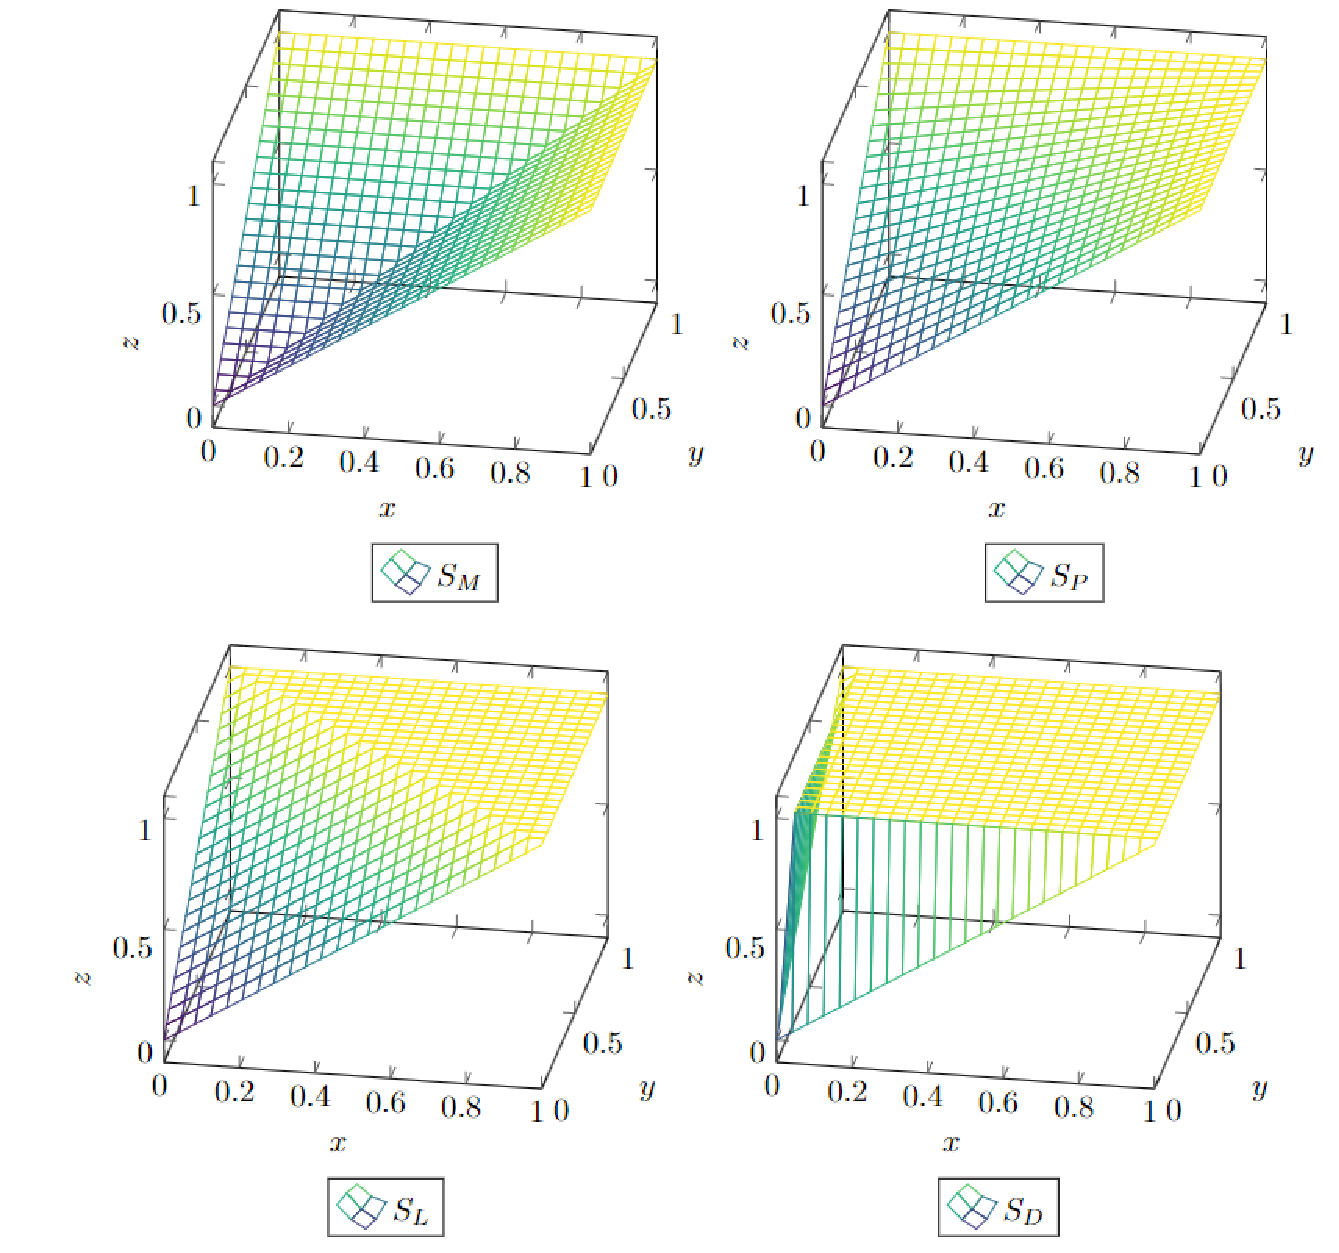
\includegraphics[scale=0.5]{template-fig/konormy.pdf}
                \centering
            \end{figure}

\end{graph}

Je zajímavé sledovat podobnosti v grafické reprezentaci t-norem a t-konorem, kde je zřetelnější komplementárnost těchto operací.

\subsection{Fuzzy implikace} 


Fuzzy implikace patří mezi nejd\r uležitější fuzzy pojmy a díky takovým spojením výrok\r u je možné mnohem jednodušeji popsat lidské vyjadřování matematicky. Implikace se v obecném jazyce vyjadřuje mnoha zp\r usoby, nejtypičtěji pak slovním spojením \textit{když-tak}. Fuzzy implikace je, podobn\v e jako p\v redchoz\'i logick\'e spojky, monot\'onn\'im roz\v s\'i\v ren\'im klasick\'e implikace.
\begin{definition} \label{impl}
    Zobrazení $I: [0,1]^2 \rightarrow [0,1] $ se nazývá implikátor, pokud
    \begin{itemize}
        \item $I$ je nerostoucí ve svojí první souřadnici,
        \item $I$ je neklesající ve svojí druhé souřadnici,
        \item $I(1,0) = 0, I(0,0) =  I(0,1) = I(1,1) = 1.$
    \end{itemize}
\end{definition}

Modelov\'an\'i fuzzy implikace je ale o něco složitější, než modelov\'an\'i dříve zmíněných logických spojek. Tyto spojky ale mohou být využity pro konstrukci fuzzy implikace. Zřejmě jsou následující logické formule tautologicky ekvivalentní: $$ p\implies q, \mbox{   } \neg p \vee q, \mbox{   } \neg p\vee (p\wedge q) .$$ Lze tedy spojit informace o modelov\'an\'i p\v redchozích logických spojek a jejich vzájemných ekvivalentních \' upravách pro tvorbu fuzzy implikátoru. Konstrukce konjunkce lze vyjádřit t-normou, diskunkce t-konormou a negace standardn\'im negátorem. Vzniknou pak n\'asleduj\'ic\'i p\v redpisy:
$$I(x,y)=S(N(x),y)\text{ neboli (S,N)-implikátory},$$
$$I(x,y)=S(N(x),T(x,y)) \text{ neboli Q-implikátory}.$$

\begin{definition}
    \cite{Springer}
    Funkce $I: [0,1]^2 \rightarrow [0,1]$ se nazývá (S,N)-implikace, pokud existuje t-konorma S a fuzzy negace N taková, že $$I(x,y) = S(N(x),y), x \in [0,1].$$
\end{definition}

\begin{example}
\cite{Springer}
Pro základní t-konormy zmíněné v kapitole \ref{sec: Triangulární konormy} a standardní negátor $N_S$ existují následující implikátory, které patří do skupiny $(S,N)-$implikátor\r u:\\
    \vbox{$$ I_{S_M}(x,y)=\max(1-x,y),$$ }
\vbox{$$ I_{S_P}(x,y)=1-x+x.y,$$}
 \vbox{$$ I_{S_L}(x,y)=\min(1-x+y,1),$$}
 $$ I_{S_D}(x,y)=\begin{cases} 1-x,
&\mbox {pokud y=0,} \\y, &\mbox {pokud x=1}, \\
1, &\mbox {jinak.} \end{cases} $$
\end{example}

Pro představu jsou níže představeny grafy implikátorů $I_{S_M}, I_{S_P}, I_{S_L}$ a $I_{S_D}.$


\begin{graph} Uk\' azka implik\' ator\r u.
    \begin{figure}[H]
                \hspace{-1cm}
                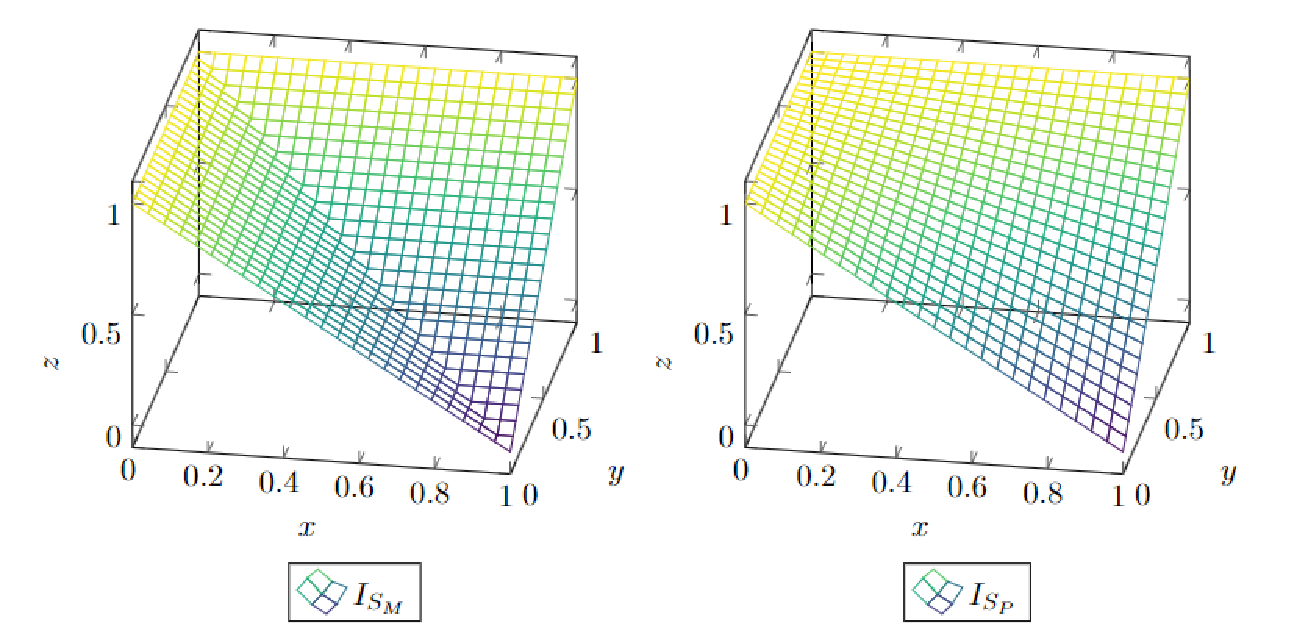
\includegraphics[scale=0.65]{template-fig/impl1.pdf}
                \centering
            \end{figure}
            \begin{figure}[H]
                \hspace{-1cm}
                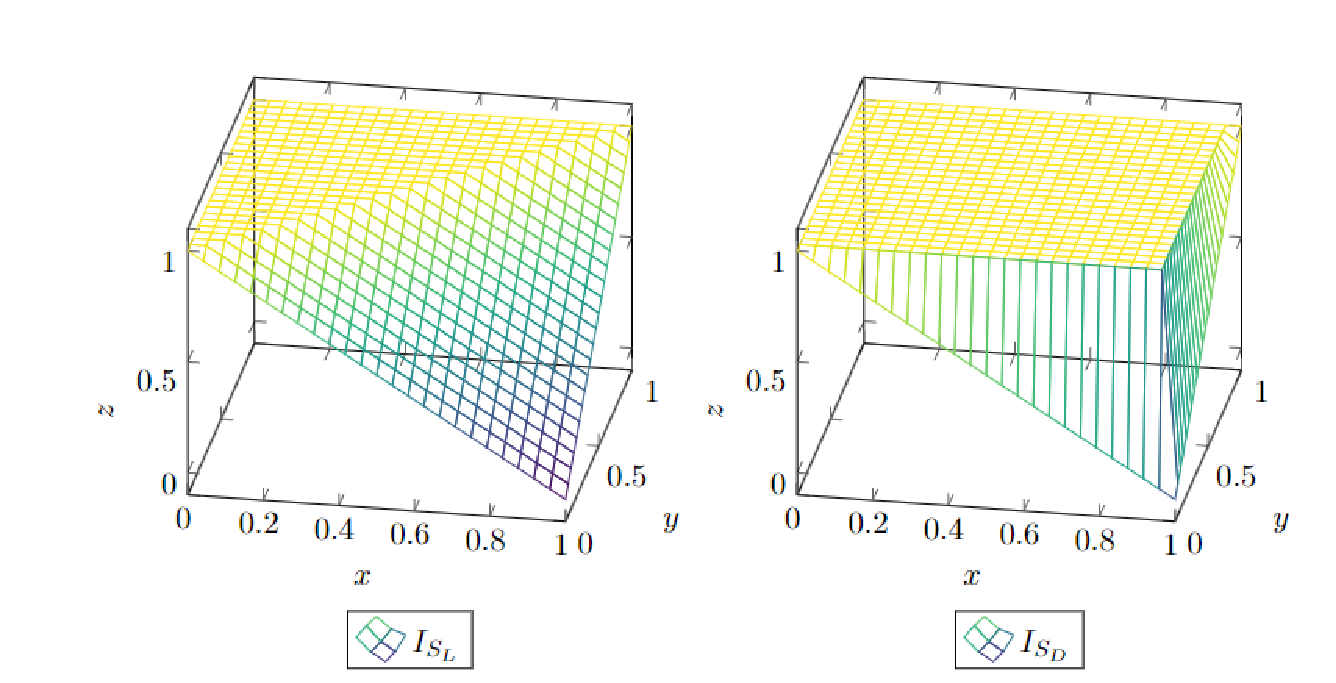
\includegraphics[scale=0.65]{template-fig/impl2.pdf}
                \centering
            \end{figure}

\end{graph}
Na tomto obrázku je možné pozorovat nápadnou podobnost s grafy t-konorem. Funkce jsou otočeny o 90 ° doleva, což jen ukazuje použití klasick\' eho negátoru ku základním t-konormám. 


Dále je nutné popsat již dříve zmíněné Q-implikátory.
\begin{definition}
    \cite{Springer}
    Funkce $I: [0,1]^2 \rightarrow [0,1]$ se nazývá Q-implikace, pokud existuje t-norma T, t-konorma S a fuzzy negace N taková, že $$I(x,y) = S(N(x),T(x,y)), x \in [0,1].$$
\end{definition}
Mezi nejznámější Q-implikátor patří tzv. Zadeh\r uv implikátor, který staví na minimové t-normě $T_M,$ maximové t-konormě $S_M$ a Zadehově negaci $N_S$. Jeho předpis pak vypadá následovně $$I_Z(x,y) = \max(1-x, \min(x,y)).$$ Podobně pak lze tvořit i další implikátory, které jsou založeny standardním negátoru a předchozích t-normách a t-konormách. Implikátor $I_P$ je tvořen součinovou t-normou $T_P,$ pravděpodobnostním součtem $S_P,$ negací $N_S$ a má předpis $$I_P(x,y) = 1-x+x^2y.$$  Po použití Łukasiewiczovy t-normy $T_L,$ Łukasiewiczovy t-konormy $S_L,$ a negátoru $N_S$ bude výsledkem klasický S-implikátor s předpisem $$I_L(x,y) = \max(1-x, y).$$ V neposlední řadě stojí za zmínku implikátor $I_D,$ který sestává z drastického součinu $T_D,$ drastického součtu $S_D,$ negátoru $N_S$ a vypadá následovně $$I_D(x,y) = \begin{cases}  y, & \mbox{pokud } x = 1,\\
                1 - x, &  jinak.  \end{cases}$$\\ 
Podobným zp\r usobem je samozřejmě možné tvořit nekonečné množství implikací s r\r uznými předpisy, které se budou měnit na základě kombinací t-norem, t-konorem a negátor\r u. Pro lepší pochopení jsou níže vykresleny grafy uvedených implikací.
\begin{graph}Implikátory $I_Z, I_P, I_L, I_D.$
\begin{figure}[H]
                \hspace{-1cm}
                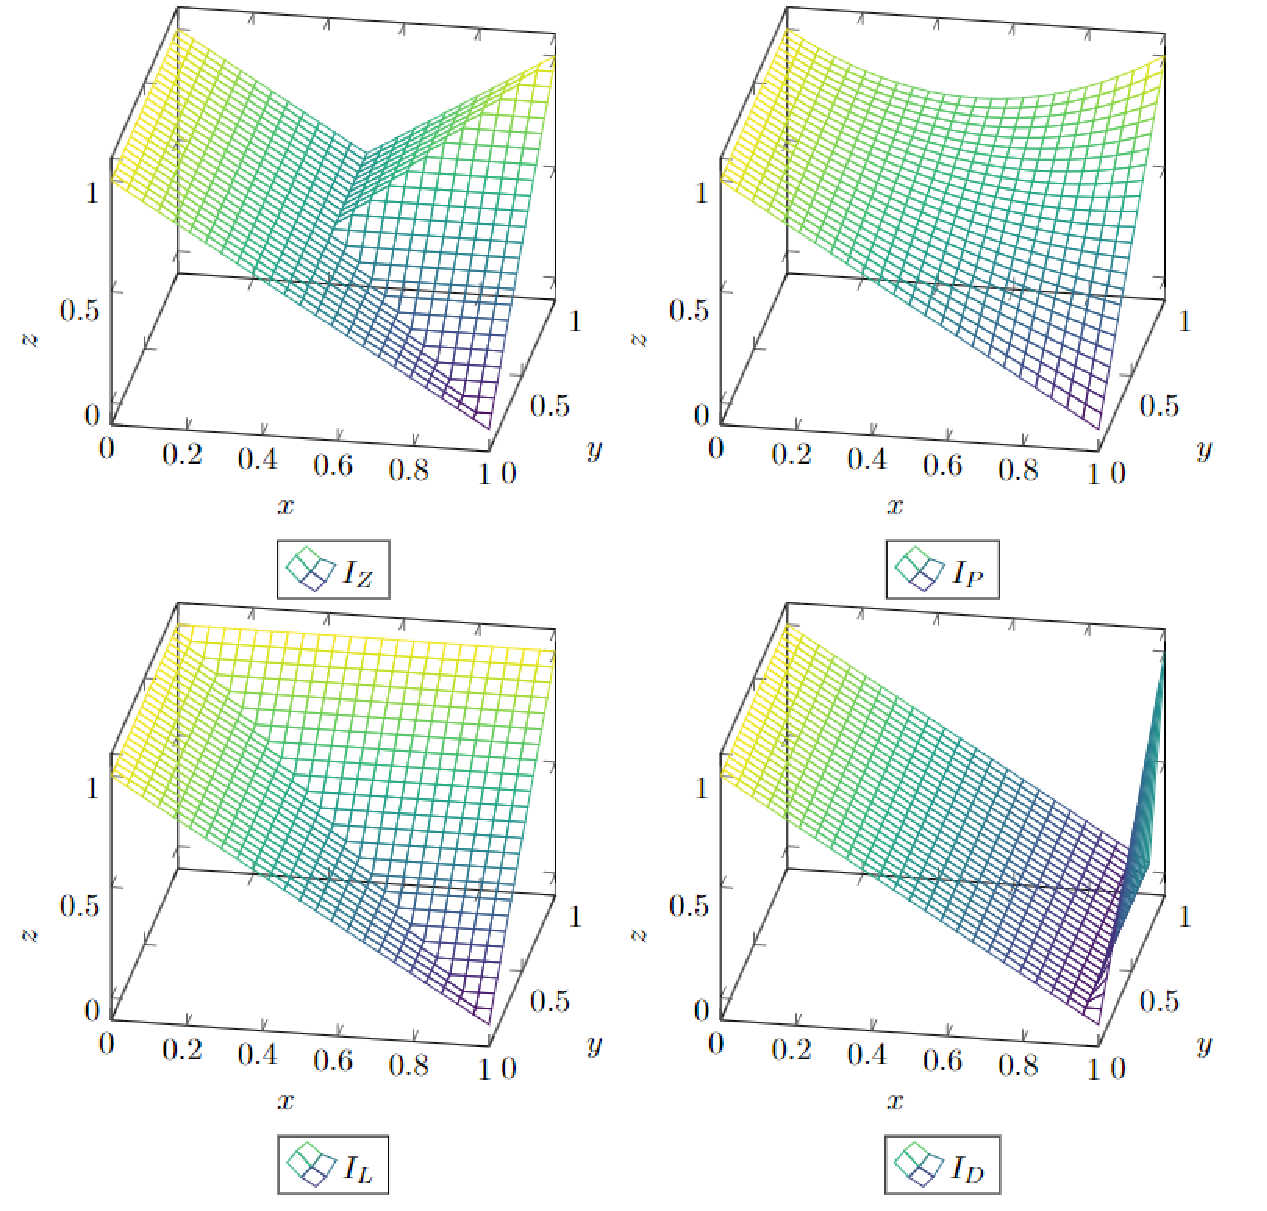
\includegraphics[scale=0.5]{template-fig/impl3.pdf}
                \centering
            \end{figure}
    
\end{graph}

Mezi nejpoužívanější rozšíření klasické implikace na interval $[0,1]$ je \textit{reziduální operátor} $R_T$ pro danou zleva-spojitou t-normu $T$, také označován jako $R-$implikátor: $$ R_T(x,y)=\sup(z \in [0,1]; T(x,z) \leq y).$$

V následujícím příkladu jsou rezidu\'aln\'i implik\'atry odvozen\'e ze zn\'am\'ych zleva spojit\'ych t-norem:
\begin{example} Pro zleva spojité t-normy $T_M, T_P$ a $T_L$ pak dostáváme  následující reziduální implikátory:
    \cite{Springer}\\
     $$ R_{T_M}(x,y)=\begin{cases} 1, &\mbox {pokud $x\leq y$,} \\y, &\mbox{jinak,} \end{cases} $$
    (Göddel\r uv implik\' ator)
     $$ R_{T_P}(x,y)=\min \left (\frac yx,1 \right ),$$
    (Goguen\r uv implikátor)
     $$ R_{T_L}(x,y)=\min(1-x+y,1).$$
    (\L{}ukasiewicz\r uv implikátor)\\
\end{example}
\begin{graph}
     Grafické znázornění R-implikátor\r u.\\
\begin{figure}[H]
                \hspace{-1cm}
                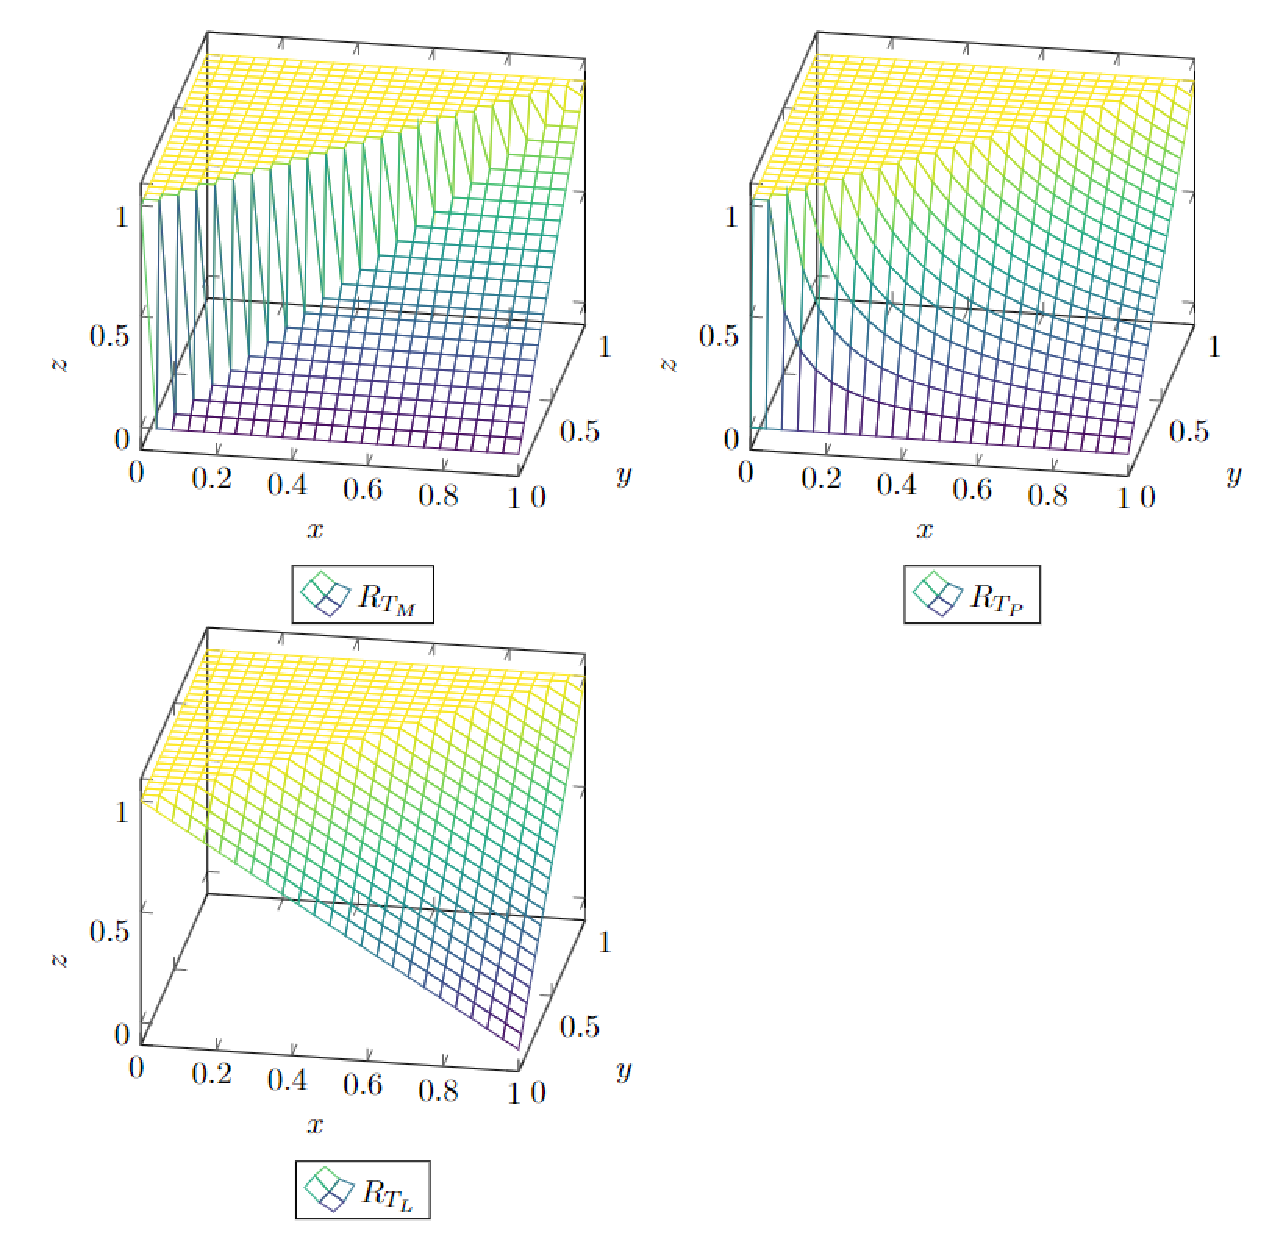
\includegraphics[scale=0.7]{template-fig/impl4.pdf}
                \centering
            \end{figure}
     

\end{graph}



Z uveden\'eho je z\v rejm\'e, \v ze fuzzy implikace jsou funkce dvou prom\v enn\'ych.
V klasick\'e logice m\'a implikace r\r uzn\'e vlastnosti, kter\'e nemus\'i tyto funkce nutn\v e spl\v novat, p\v ritom spl\v nuj\'i v\v sechny podm\'inky z Definice \ref{impl}.

\begin{definition}
\cite{Springer}
Říká se, že fuzzy implik\'ator $I:[0,1]^2 \rightarrow [0,1]$ spl\v nuje:
\begin{enumerate}
\item[(NP)] levý princip neutrality, pokud
$$I(1,y)=y; ~~~~y \in [0,1],$$
\item[(EP)] princip z\'aměny, pokud
$$I(x,I(y,z))=I(y,I(x,z)) \mbox{  pro ka\v zd\'e   } x,y,z \in [0,1],$$
\item[(IP)] princip identity, pokud
$$I(x,x) = 1; ~~~ x \in [0,1], $$
\item[(OP)] vlastnost uspořádání
$$x \leq y \iff I(x,y) =1; ~~~ x,y \in [0,1],$$
\item[(CP)] kontrapozitivitu vzhledem na dan\'y neg\'ator $N$, pokud
$$ I(x,y)=I(N(y),N(x)); ~~~ x,y \in [0,1],$$
 {\item[(LI)] z\'akon přenosu  vzhledem na  t-normu $T$, pokud
$$I(T(x, y), z) = I(x, I(y, z)); ~~~ x,y,z \in  [0, 1],$$
\item[(WLI)]  slab\'y z\'akon přenosu vzhledem na komutativní a
rostoucí funkci $F:
[0,1]^2 \to [0, 1]$, pokud
$$I(F(x, y), z) = I(x, I(y, z)); ~~~  x,y,z \in  [0, 1].$$}
\end{enumerate}
\end{definition}

\begin{remark}
    Bylo dok\'az\'ano, \v ze nap\v r. (S,N)-implikátory spl\v nují v\v zdy $(NP)$ a $(EP)$, reziduální implikátor zase spl\v nuje v\v zdy $(NP)$ a $(OP).$
\end{remark}

\subsection{Konstrukce fuzzy implikátor\r u}

Většina implikátor\r u je ve fuzzy logice modelována pomocí t-norem. Konstrukce nových t-norem, tedy nových konjunktor\r u, je naznačena v předchozích kapitolách. Při konstruování implikátor\r u lze použít podobný postup.

Generování implikátor\r u lze rozdělit do tří tříd. Yager popsal první dvě třídy, tedy $f-$generované a $g-$generované implikátory. Za popsání  $h-$generovaných implikátor\r u, tedy poslední třídy, si připisuje zásluhy Balasubramaniam Jayram. Následně jsou všechny třídy představeny.

\begin{sentence}\cite{yager} 
Pokud je $f: [0,1] \to [0,\infty]$ klesající a spojitá funkce,
přičemž $f(1) = 0,$ potom je funkce $I: [0,1]^2 \to [0,1],$ dána předpisem
$$I(x,y) = f^{-1}(x \cdot f(y)), \mbox {   } x, y \in [0,1],$$
fuzzy implikátor (pričemž $0 \cdot \infty = 0$). \\
\end{sentence}

\begin{example}
    \cite{Springer}
    Konstrukce f-generovaných implikátor\r u m\r uže vypadat následovně.
    Pokud by byl použit aditivní generátor součinové t-normy $T_P,$ tedy 
    pokud $f(x) = - \log x,$ výsledkem bude Yager\r uv implikátor:
    $$I_{YG}(x,y)= \begin{cases} 1,
    &\mbox {pokud $x=0$ a $y=0,$} \\
    y^x, &\mbox {jinak.}
    \end{cases}$$
\end{example}
\begin{remark}
    V předchozím příkladu se nejednalo o $(S,N)-$implikátor ani o R-implikátor. To však neplatí pro všechny f-generované implikátory.
\end{remark}


\begin{sentence}\cite{yager} 
Pokud je $g: [0,1] \to [0,\infty]$ klesající a spojitá funkce,
přičemž $g(1) = 0,$ potom je funkce $I: [0,1]^2 \to [0,1],$ dána předpisem
$$I(x,y) = g^{(-1)}\left (\frac 1x \cdot g(y)\right ), \mbox {   } x, y \in [0,1]$$
fuzzy implikátor (pričemž $\frac{1}{0} = \infty, 0 \cdot \infty = 0$). \\
\end{sentence}
\begin{example}
    \cite{Springer}
    Pokud by byl použit aditivní generátor pravděpodobnostního součtu $S_P,$ tedy 
    pokud $g(x) = - \log (1- x),$ dostaneme následující fuzzy implikátor:
    $$I_{YG}(x,y)= \begin{cases} 1,
    &\mbox {pokud $x=0$ a $y=0,$} \\
    1-(1-y)^x, &\mbox {jinak.}
        \end{cases}$$
\end{example}
\begin{remark}
    Opět se v předchozím příkladu nejednalo o $(S,N)-$implikátor ani o R-implikátor. To však také neplatí v každém případě g-generovaných implikátor\r u.
\end{remark}

\begin{sentence}\cite{Springer} 
Pokud je $h: [0,1] \to [0,\infty]$ klesající a spojitá funkce,
přičemž $h(1) = 0,$ potom je funkce $I: [0,1]^2 \to [0,1],$ dána předpisem
$$I(x,y) = h^{(-1)}(x \cdot h(y)), \mbox {   } x, y \in [0,1]$$
fuzzy implikátor. \\
\end{sentence}
\begin{example}
    Pokud by byl jako  $h-$generátor funkce $h_n(x) = 1- \frac {x^n}{n}, n
    \in N,$ výsledkem budou následující fuzzy implikátory:
    $$I_n(x,y) = \min \left ( (n - n \cdot x + x \cdot y^n)^{\frac 1n}, 1\right
    ),$$
    kter\'e jsou $(S,N)-$implikátory.
\end{example}
\begin{remark}
    Pro h-negátory platí, že $I_{h_1} = I_{h_2}$ právě když $h_1 = h_2.$
\end{remark}

Všechny třídy generátor\r u jsou, stejně jako v případě spojitých aditivních generátor\r u, jednoznačně dané s proměnlivou kladnou konstantou.

Krom\v e uveden\'ych zp\r usob\r u byly pops\'any i dal\v s\'i konstrukce implik\'ator\r u, n\v ekter\'e zde tak\'e uv\'ad\'ime.

\begin{sentence}
\cite{Springer}
    Nech\v t je  $f:[0,1]\rightarrow [0,\infty]$ klesající funkce taková, \v ze $f(1)=0$. 
Potom funkce $I_f(x,y):[0,1]^2\rightarrow [0,1]$ dan\'a předpisem
 $$I_f(x,y)=\begin{cases} 1 & \mbox{pokud $x \leq y$},\\
f^{(-1)}(f(y^+)-f(x)) & \mbox{jinak,} \end{cases}$$
kde $f(y^+)= \lim\limits_{y \to y^+}f(y)$ a $f(1^+)=f(1)$
je fuzzy implik\'ator. \\
\end{sentence}

Následuje ilustrační příklad třídy generovaných implikátor\r u.\\
\begin{example}
    Nech\v t je $f_1:[0,1] \rightarrow [0,
\infty]$ funkce daná předpisem:
 $$f_1(x)= -\ln(x).$$

Je d\r uležité zmínit, že je funkce klesající. Pro $f_1^{(-1)}$ pak platí:
 $$f_1^{(-1)}(x)=\min \{ e^{-x},1 \}.$$
Pro  funkci $f_1$ pak lze dostat následující implik\'ator:
$$I_{f_1}(x,y)= \begin{cases} 1,    &\mbox{pokud $x \leq y$}, \\
  \frac{y}{x},   & \mbox{jinak.} \end{cases}$$
\end{example}


Dalším typem generovaných implikátor\r u jsou $I^g$ implikátory. Narozdíl od $I_f$ implikátor\r u jsou ale generovány rostoucími funkcemi.

\begin{sentence} \cite{smutna}
    Nech\v t je  $g:[0,1]\rightarrow [0,\infty]$ rostoucí funkce takov\'a, \v ze $g(0)=0$. 
    Potom funkce $I^g(x,y):[0,1]^2 \rightarrow [0,1]$ dan\'a předpisem
    %\begin{equation}\label{g}
    $$I^g(x,y)=g^{(-1)}(g(1-x)+g(y)),$$
    %\end{equation}
    je fuzzy implik\'ator.\\
\end{sentence}

\begin{example}
\cite{Springer}
    Nech\v t jsou $g_1, g_2:[0,1] \rightarrow [0,\infty]$ 
    dan\'e předpisy:
    \begin{itemize}
    \item $g_1(x)=\begin{cases}  x,    &\mbox{pokud $x \leq 0.5$}, \\
    0.5+0.5x,      &\text{jinak,} \end{cases}$
    \item $g_2(x)=-\ln(1-x).$
    \end{itemize}
    Obě dvě funkce $g_1$ a $g_2$ josu rostoucí.
    Pro jejich pseudo-inverzn\'i funkce  $g_1^{(-1)}$ a $g_2^{(-1)}$ plat\'i:
    \begin{itemize}
    \item $g_1^{(-1)}(x)=\begin{cases} x, &\mbox{pokud $x \leq 0,5$}, \\
    0,5,   &\mbox{pokud $0,5 < x \leq 0,75$}, \\
    2x-1,   &\mbox{pokud $0,75 < x \leq 1$}, \\
    1,   &\mbox{pokud $1 < x$}, \end{cases}$
    \item $g_2^{(-1)}(x)=1-e^{-x} ~ \mbox{pro $x \in [0, \infty]$}.$
    \end{itemize}
    Potom se pro funkce $g_1$ a $g_2$ modelují nasleduj\'icí implik\'atory:
    \begin{itemize}
    \item $I^{g_1}(x,y)=\begin{cases}  1-x+y,      &\mbox{pokud $x \geq 0.5, y \leq 0.5, x-y \geq 0.5$}, \\
    0.5,      &\mbox{pokud $x \geq 0.5, y \leq 0.5, 0.25 \leq x-y < 0.5$}, \\
    1-2x+2y,      &\mbox{pokud $x \geq 0.5, y \leq 0.5, x-y < 0.25$}, \\
    \min(1-x+2y,1),       &\mbox{pokud $x < 0.5, y \leq 0.5$}, \\
    \min(2-2x+y,1),       &\mbox{pokud $x \geq 0.5, y>0.5$}, \\
    1,       &\mbox{pokud $x < 0.5, y > 0.5,$} \end{cases}$
    \item $I^{g_2}(x,y)=1-e^{\ln(x(1-y))}=1-x+xy.$
    \end{itemize}
\end{example}

\begin{sentence} \cite{habilitace}
    Nech\v t je $c$ kladn\'a konstanta a $g:[0,1] \to [0,\infty]$
    rostoucí  funkce. Potom implik\'atory $I^g$ a $I^{c \cdot g}$,
    které jsou zalo\v zen\'e na  funkcích $g$ a $c \cdot g$, jsou
    identick\'e.
\end{sentence}
A na z\'av\v er uvedeme zp\r usob konstrukce, s kter\'ym jsme se potkali p\v ri konstrukci t-norem.

\begin{sentence}\cite{Springer}
    Nech\v t $\varphi \in B$, potom pro libovolný implikátor $I: [0,1]^2 \rightarrow [0,1]$ je $\varphi$-transformace $I_\varphi$ také implikátor.
\end{sentence}

\begin{definition}\cite{Springer}
    Nech\v t je $\varphi:[0,1] \rightarrow [0,1]$  rostoucí
    bijekce a množina všech takových bijekcí Nech\v t je B. Nech\v t je funkce
    $I:[0,1]^2\rightarrow [0,1]$ 
    implikátor.
    Pak je funkce
    $$I_\varphi(x,y)=\varphi^{-1}(I(\varphi (x), \varphi (y)))$$
    $\varphi-${\em transformací implikátoru} $I.$ Implikátor se nazývá
    {\em totálně invariantní,} pokud pro libovolnou funkci $\varphi \in B$ platí $I_\varphi=I.$\\
\end{definition}

\section{Konstrukce fuzzy logick\'ych spojek}

V této kapitole se věnuji konstrukci fuzzy logických spojek pomocí funkcí jedné proměnné a již existujících spojek. Dále tyto poznatky budou využity při analýze lidského vyjadřování v běžném jazyce a při konstrukci fuzzy logických spojek na něm založených.

\subsection{$\varphi-$transformace triangulárních norem a konorem}

Následující část se věnuje zobecn\v en\'i $\varphi-$transformaci t-norem, konkr\'etn\v e $\varphi-$transformaci $T_M.$ Zobecn\v en\'i bude spo\v c\'ivat v tom, \v ze funkce $\varphi$ nebude rostouc\'i bijekce, bude to jenom neklesaj\'ici funkce, proto zde tak\'e vyu\v zijeme zobecn\v en\'i inverzn\'i funkce. 
\begin{sentence}\cite{KMP}\label{subnorma}
     Nech\v t je $\varphi : [0,1] \rightarrow [0,1]$ neklesající funkce a  spojitá na otev\v ren\'em intervalu
 $]0,1[$ a nech\v t $T: [0,1]^2 \rightarrow [0,1]$ je t-norma. Potom funkce
    $(T)_\varphi : [0,1]^2 \rightarrow [0,1]$ je dána p\v redpisem $$(T)_\varphi (x,y)= \begin{cases} \min(x,y), & \mbox {pokud } \max(x,y) = 1,
    \\ \varphi^{(-1)}[T(\varphi(x), \varphi(y))], & \mbox {jinak,}
    \end{cases}$$
    je t-norma.
  \end{sentence}
  V této práci se blí\v ze seznámíme s $\varphi-$transformaci $T_M$ a využijeme zobecnění předchozí věty:

\begin{sentence} 
\cite{hlinena}
\label{smut} Nech\v t je $\varphi \colon [0,1] \to [0,1]$ neklesající funkce. Pak je funkce $(T_M)_\varphi\colon[0,1]^2\to[0,1]$  t-normou pouze v případě, že
$$\varphi^{(-1)}\circ\varphi\circ\varphi^{(-1)}\circ\varphi(x)\in \{\varphi^{(-1)}\circ\varphi(x),\varphi^{(-1)}\circ\varphi\circ\varphi^{(-1)}\circ\varphi(1^-)\}$$
pro každé $x\in[0,1],$ kde $\varphi^{(-1)}\circ\varphi\circ\varphi^{(-1)}\circ\varphi(1^-)=\lim\limits_{x\to 1^-}\varphi^{(-1)}\circ\varphi\circ\varphi^{(-1)}\circ\varphi(1^-).$
\end{sentence}
\begin{remark}
\cite{mitav}
    Nech\v t $\varphi\colon[0,1]\to [0,1]$ je neklesající, zleva spojitá  funkce a nechť $a=\inf\{x \in [0,1]\colon \varphi(x)=1\}.$ Potom operace $(T_M)_\varphi\colon[0,1]^2\to[0,1]$ je t-normou právě když platí $\varphi^{(-1)}\circ\varphi\circ\varphi^{(-1)}\circ\varphi(x)=\varphi^{(-1)}\circ\varphi(x)$ pro každé $x \in [0,a].$ Tato  t-norma je zleva spojitá na intervalu  $]0,1[^2$, ale není zleva spojitá na  intervalu $[0,1]^2.$
\end{remark}

Uveden\'e podm\'inky znamenaj\'i, \v ze funkce $\varphi$ nem\r u\v ze m\'it dva konstantn\'i \'useky v bezprost\v redn\'i bl\'izkosti. P\v ri poru\v sen\'i t\'eto podm\'inky by v\'ysledn\'a funkce nebyla asociativn\'i.
\bigskip


  
  N\'asleduj\'ic\'i p\v r\'iklad objas\v nuje situaci pro $T_M$ a jej\'i $\varphi-$transformaci, kdy\v z $\varphi$ je neklesaj\'ic\'i funkce. 
\begin{example}
\label{sub: fi}
Nech\v t $\varphi:[0,1] \to [0,1]$ je d\'ana p\v redpisem:    
 $$\varphi(x) = \begin{cases} x, & \mbox {pokud } x \in [0,\frac{1}{3}],
    \\ \frac{1}{3}, & \mbox {pokud } x \in [\frac{1}{3}, \frac{2}{3}],\\
    2x - 1, & \mbox {pokud } x \in [\frac{2}{3}, 1].
    \end{cases}$$
Potom pro $\varphi-$transformaci $T_M$ plat\'i
$$(T_M)_{\varphi(x)} = \begin{cases} \frac{1}{3}, & \mbox {pokud } (x, y) \in [\frac{1}{3},\frac{2}{3}]^2 \cup [\frac{1}{3}, \frac{2}{3}] \times [\frac{2}{3}, 1] \cup [\frac{2}{3}, 1] \times [\frac{1}{3}, \frac{2}{3}],\\
    T_M, & \mbox {jinak.}
    \end{cases}$$
\end{example}
Pro lep\v s\'i n\'azornost uv\'ad\'im graf  funkce $\varphi$ a jej\'i pseudoinverzn\'i funkce a tak\'e vizu\'aln\'i rozd\v elen\'i grafu funkce $\left(T_M\right)_\varphi.$\\
\begin{graph}
    Vizu\' aln\' i zobrazení funkce $\varphi$ a jej\'i pseudoinverzn\'i funkce
\begin{figure}[H]
                \hspace{-1cm}
                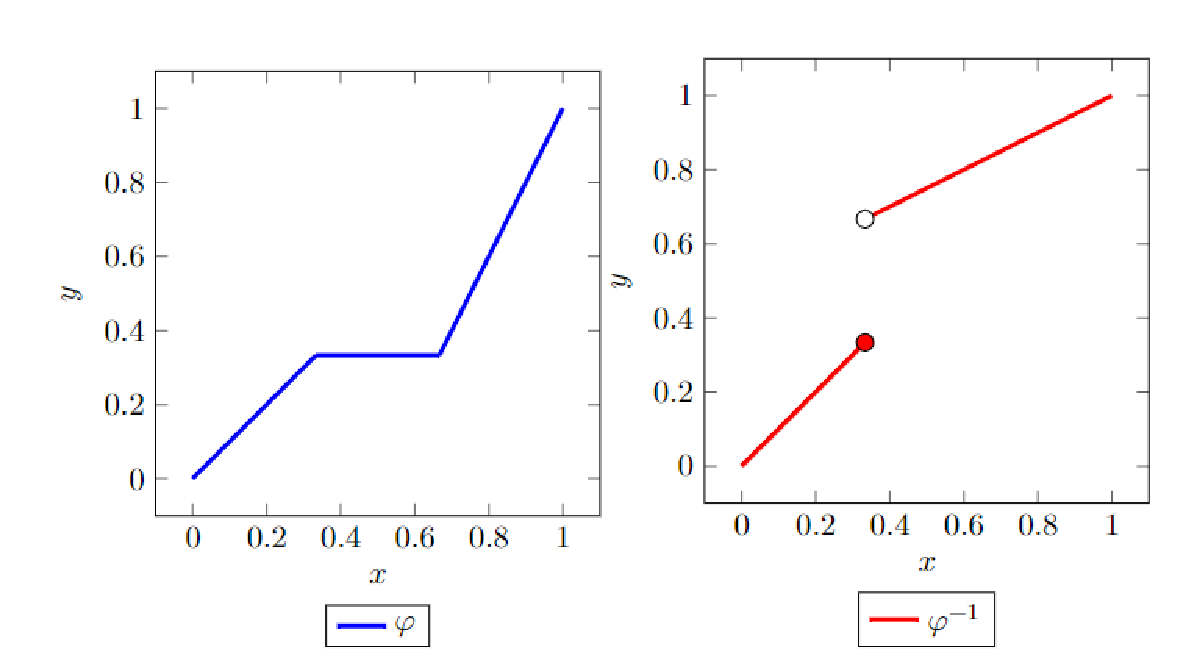
\includegraphics[scale=0.75]{template-fig/phi_transform.pdf}
                \centering
            \end{figure}
\end{graph}

    
\begin{graph}Vizu\' aln\' i rozd\v elen\'i grafu $\varphi$-transformace minimov\' e t-normy\\
\tikzset{>=stealth}
\centering
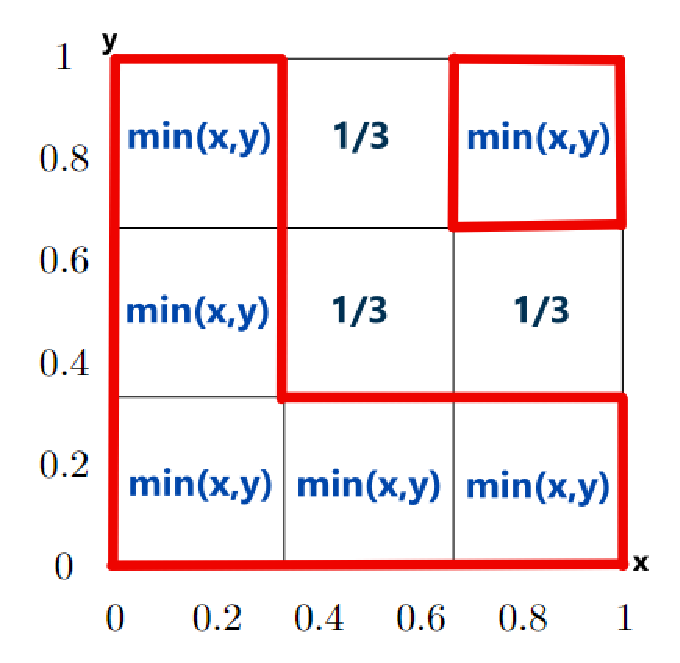
\includegraphics[scale=0.8]{template-fig/phi-tnorm.pdf}
\end{graph}

%\begin{tikzpicture}
%    \draw[step=1cm,black,thin] (0,0) grid (10,10);
%   \foreach \xtick in {0,...,10} {\pgfmathsetmacro\result{\xtick * .1} \node at (\xtick,-0.5) 
% {\pgfmathprintnumber{\result}}; }
%    \foreach \ytick in {0,...,10} {\pgfmathsetmacro\result{\ytick * .1} \node at (-.5,\ytick) 
%{\pgfmathprintnumber{\result}}; }
    
%\end{tikzpicture} 
Příklad \ref{sub: fi} nám ilustruje vliv průběhu funkce $\varphi$ na průběh t-normy, která vznikla $\varphi-$transformací. Pro obecnou funkci $\varphi$ a t-normu $T_M$ dostáváme funkci $(T_M)_{\varphi}$, předpis které popisuje následující tvrzení.
\begin{sentence}
\cite{mitav}
\label{t-norm}
 Nech\v t je $\varphi:[0,1]\rightarrow [0,1]$
neklesající funkce spojitá na otevřeném intervalu $]0,1[$.
Nech\v t je $\{[a_i,b_i]\}_{i\in I}$ množina podinterval\r u
intervalu $[0,1]$ taková, že $\varphi(x)=c_i$ pro $x\in
[a_i,b_i]$ (přičemž na intervalu $[0,1]\backslash \bigcup \limits_{i \in I}
[a_i,b_i]$ je funkce $\varphi$
rostoucí).
Pak je operátor $(T_M)_{\varphi}$  t-norma daná předpisem
$$ (T_M)_{\varphi}(x,y) = \begin{cases} \varphi^{(-1)}(c_i)=a_i, &\mbox {pokud
$(x,y)\in [a_i,1[\times[a_i,b_i]$ nebo}
\\ & (x,y)\in [a_i,b_i]\times[b_i,1[,
\\ T_M(x,y), &\mbox {jinak.}
\end{cases} $$
\end{sentence}

Na základě uvedeného předpisu lze pak sestavit obecný graf znázor\v nující pr\r uběh funkce $\varphi^{(-1)}$ a poté na ní založené t-normy. Obrázek uvádím níže.
\begin{graph}
    Příklad obecné funkce $\varphi^{(-1)}$ a obecné $\varphi$-transformace minimové t-normy.\\
    \centering
        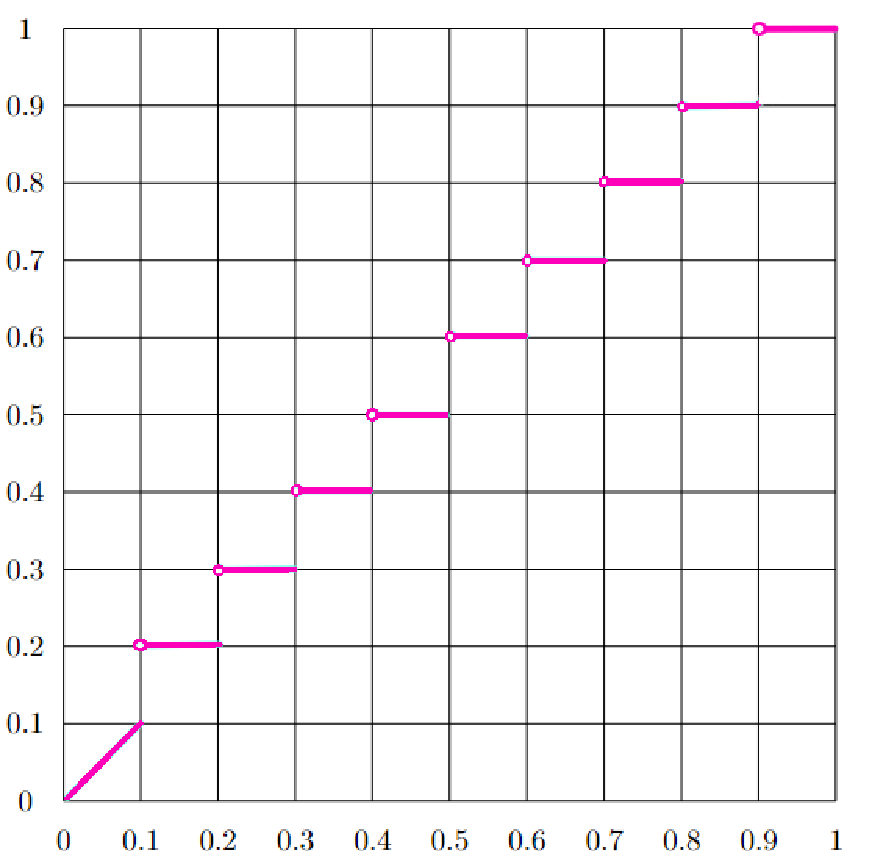
\includegraphics[scale=0.4]{template-fig/basic.pdf}
        \centering
        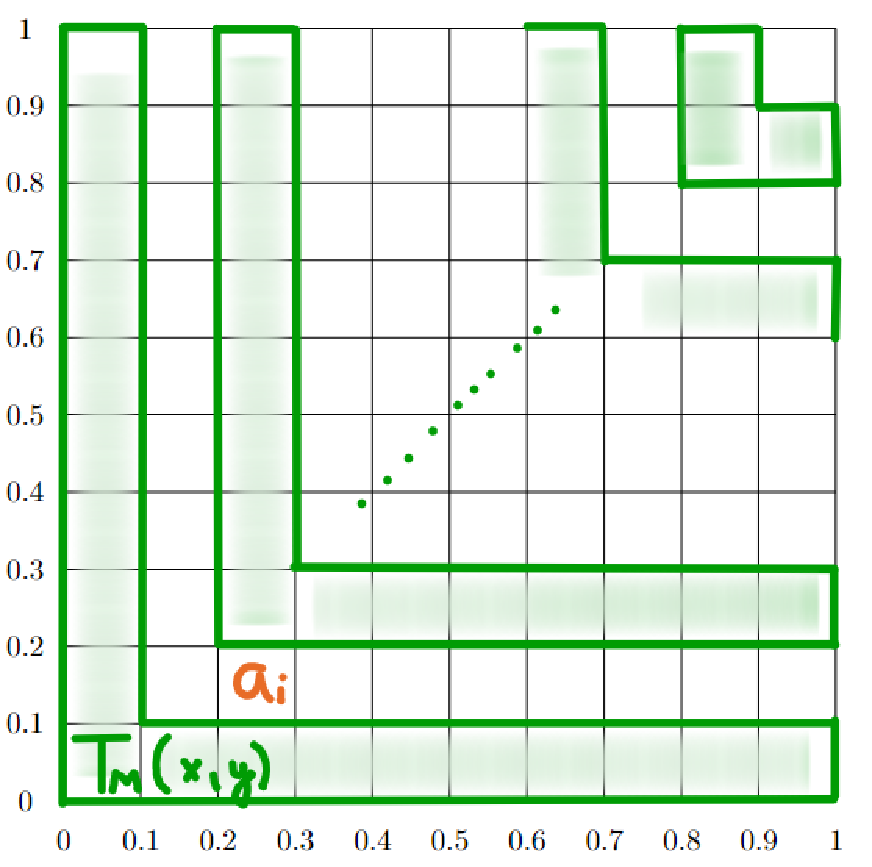
\includegraphics[scale=0.4]{template-fig/t-norma.pdf}

\end{graph}
\begin{example}
    \label{conormphi}
    Vzhledem k tomu, \v ze ke ka\v zd\'e t-norm\v e lze sestrojit jej\'i du\'aln\'i t-konormu, tak aplikujeme na $\left(T_M\right)_\varphi$ vztah $S(x,y)=1-T(1-x,1-y)$ a pro $\left(S_M\right)_\varphi$ dostaneme
 $$(S_M)_\varphi(x,y) = \begin{cases} \frac{2}{3}, & \mbox {pokud } (x,y) \in [0,\frac{1}{3}[\times[\frac{1}{3},\frac{2}{3}] \cup [\frac{1}{3},\frac{2}{3}]\times[0,\frac{1}{3}[ \cup [\frac{1}{3},\frac{2}{3}]^2,
    \\ S_M, & \mbox {jinak. }
    \end{cases}$$
    \begin{graph}Vizu\' aln\' i rozd\v elen\'i grafu $\varphi$-transformace maximové t-konormy
    \label{graph: max-conorm}


\centering
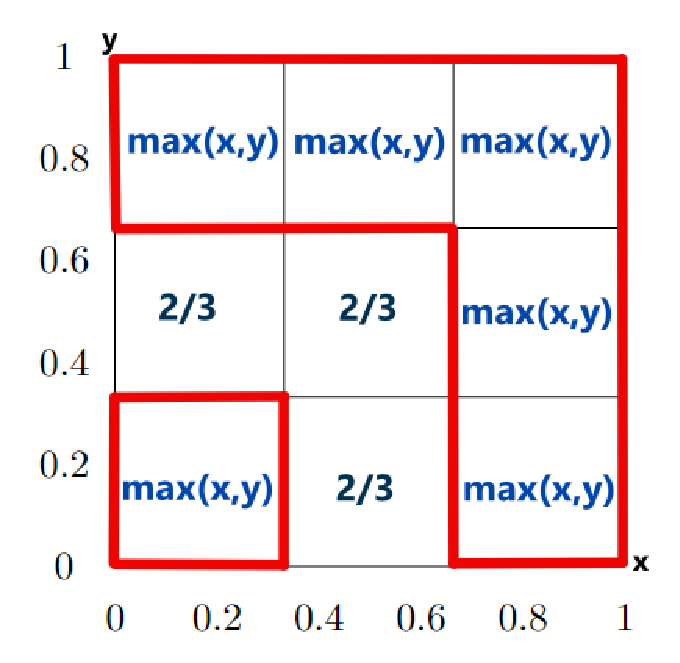
\includegraphics[scale=0.8]{template-fig/phi-t-conorm.pdf}
\end{graph}

\end{example}
Příklad \ref{conormphi} nám ilustruje vliv průběhu funkce $\varphi$ na průběh t-konormy, která vznikla $\varphi-$transformací. Pro obecnou funkci $\varphi$ a t-konormu $S_M$ dostáváme funkci $(S_M)_{\varphi}$, předpis které popisuje následující tvrzení.

\begin{sentence}
\cite{mitav}
    \label{t-conorm}
 Nech\v t je $\varphi:[0,1]\rightarrow [0,1]$
neklesající funkce spojitá na otevřeném intervalu $]0,1[$.
Nech\v t je $\{[a_i,b_i]\}_{i\in I}$ množina podinterval\r u
intervalu $[0,1]$ taková, že $\varphi(x)=c_i$ pro $x\in
[a_i,b_i]$ (přičemž na intervalu $[0,1]\backslash \bigcup \limits_{i \in I}
[a_i,b_i]$ je funkce $\varphi$
rostoucí).
Pak je operátor $(S_M)_{\varphi}$  t-konorma daná předpisem
$$ (S_M)_{\varphi}(x,y) = \begin{cases} 1-\varphi^{(-1)}(c_i), &\mbox {pokud
$(x,y)\in [1-b_i,1-a_i[\times[0,1-a_i]$ nebo}
\\ & (x,y)\in [0,1-b_i]\times[1-b_i,1-a_i[,
\\ S_M(x,y), &\mbox {jinak.}
\end{cases} $$
\end{sentence}

Na základě uvedeného předpisu lze pak opět sestavit obecný graf znázor\v nující pr\r uběh t-konormy.

\begin{graph}
    Příklad obecné $\varphi$-transformace minimové t-konormy.
    \begin{figure}[H]
                \hspace{-1cm}
                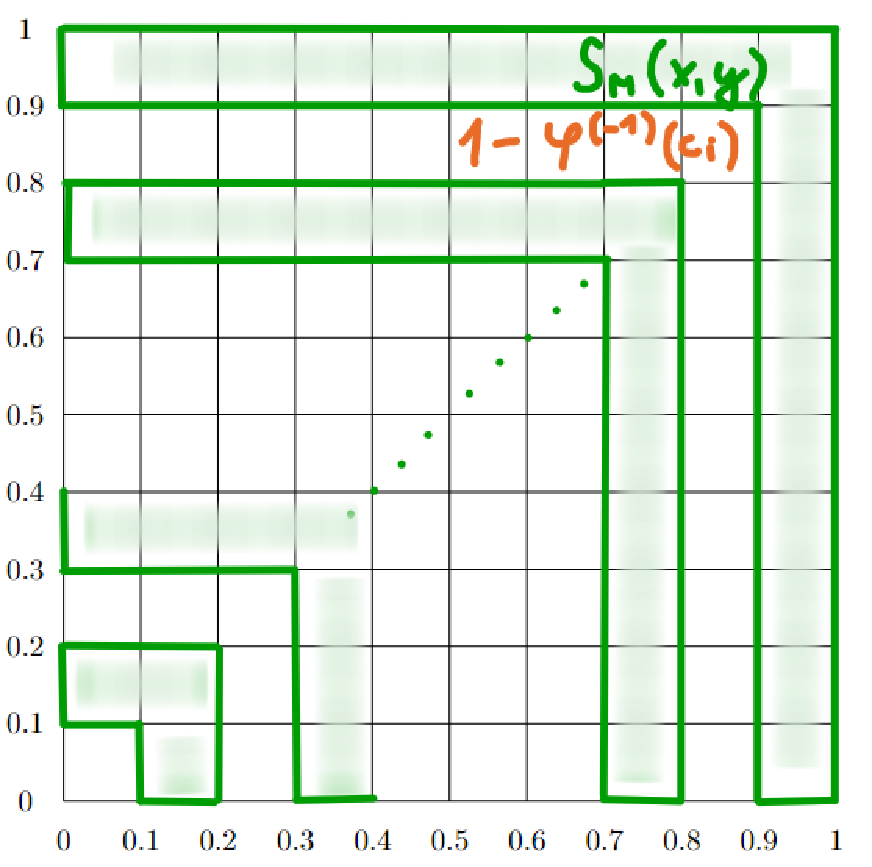
\includegraphics[scale=0.4]{template-fig/t-konorma.pdf}
                \centering
            \end{figure}
\end{graph}


\subsection{Konstrukce $(S,N)-$implik\'ator\r u pomoc\'i $\varphi-$transformace t-konorem}
 V této kapitole se věnuji konstrukcím $(S,N)-$implikací založených na standardní Zadehově negaci a $(S_M)_\varphi$, přičemž $\varphi$ je neklesající zleva spojitá funkce.
 
\begin{example}
    Nech\v t je $\varphi$ funkce z p\v ríkladu \ref{sub: fi}.  Pomocí standardní fuzzy negace $N_S(x)$ a maximové t-konormy $(S_M)_\varphi$  zkonstruujeme $(S,N)-implikaci$. 
\end{example}
   
     \begin{graph} 
     Vizu\' aln\' i rozd\v elen\'i grafu $\varphi$-transformace $(S,N)-$implikace tvořené maximovou t-konormou\\
        \centering
        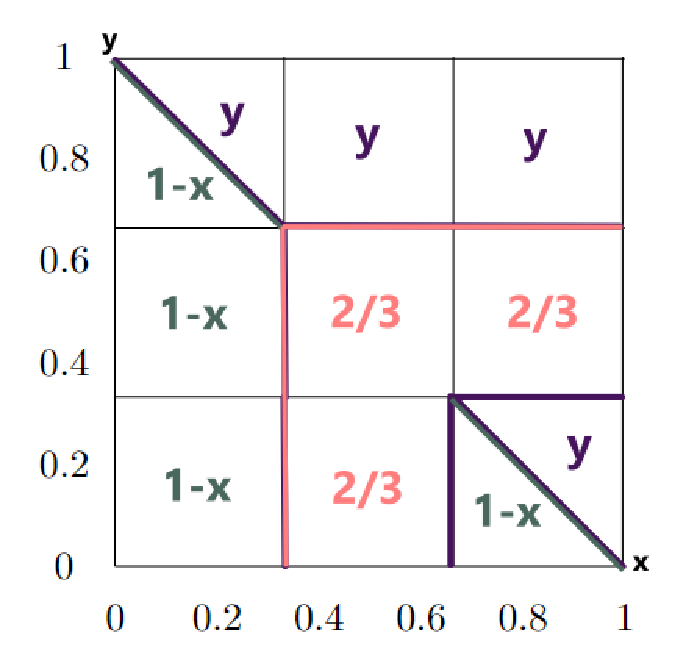
\includegraphics[scale=0.8]{template-fig/phi-impli.pdf}
    \end{graph}


 Konstrukci tohoto $(S,N)-$implikátoru lze tedy popsat následujícím předpisem:
    Nech\v t je  $\varphi:[0,1]\rightarrow [0,1]$
funkce z příkladu \ref{sub: fi}.
Potom je implikace $(S,N)-$ na základě $N_S$ a $(S_M)_{\varphi}$ dána vzorcem
$$ I_{(S_M)_{\varphi}}(x,y) = \begin{cases} \frac{2}{3}, &\mbox {pokud~~}
(x,y)\in [\frac{1}{3},\frac{2}{3}[\times[0,\frac{2}{3}] \mbox{~~nebo~~}
\\ & (x,y)\in [\frac{2}{3},1]\times[\frac{1}{3},\frac{2}{3}[,
\\ \max(1-x,y), &\mbox {jinak.}
\end{cases} $$

Pro obecnou neklesající a zleva spojitou funkci $\varphi$, standardní negátor a maximovou t-konormu dostáváme fuzzy implikátor, kterého obecný předpis je v následujícím tvrzení.
\begin{sentence}
\cite{mitav}
\label{sn-impl}
       Nechť $\varphi:[0,1]\rightarrow [0,1]$
je neklesající a zleva spojitá funkce na intervalu $]0,1[$.
Nechť
$\{[a_i,b_i]\}_{i\in I}$ je množina podintervalů intevalu $[0,1]$, přičemž $\varphi(x)=c_i$ pro $x\in
[a_i,b_i]$.
Potom $(S,N)-$implikátor založený na $N_S$ a $(S_M)_{\varphi}$ je dán formulí
$$ I_{(S_M)_{\varphi}}(x,y) = \begin{cases} 1-\varphi^{(-1)}(c_i)=1-a_i, &\mbox {~~pokud~~}
(x,y)\in [a_i,b_i[\times[0,1-a_i] \mbox{~~nebo~~}
\\ & (x,y)\in [b_i,1]\times[1-b_i,1-a_i[,
\\ \max(1-x,y), &\mbox {jinak.}
\end{cases} $$

\end{sentence}

Obecný průběh takového implikátoru pak lze vyjádřit následujícím grafem:
\begin{graph}
    Příklad obecného $(S,N)-$implikátoru $I_{(S_M)_{\varphi}}$.
            \begin{figure}[H]
                \hspace{-1cm}
                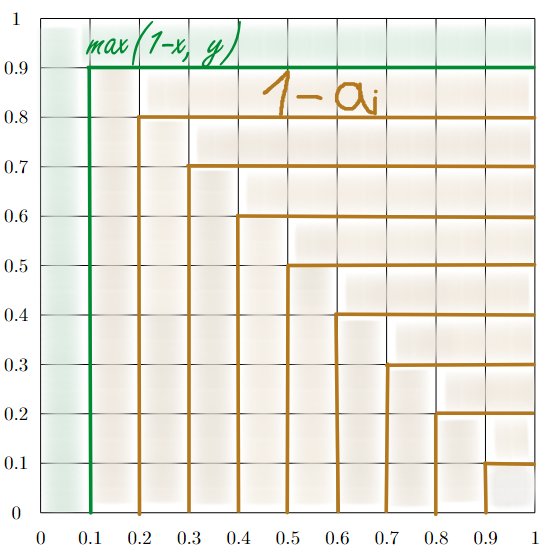
\includegraphics[scale=0.5]{template-fig/sn-implphi.PNG}
                \centering
            \end{figure}
\end{graph}

\subsubsection{Nová třída fuzzy implikací}
Mějme nějakou funkci $\varphi$, jež nebude spl\v novat podmínku z Věty \ref{smut}. Pak $(S_M)_{\varphi}$ nebude asociativní, ale bude stále fuzzy disjunkcí $D.$ Použitím konstrukce $D(N_s(x),y)$ dostaneme implikaci, která bude mít velmi podobné vlastnosti jako klasické $(S,N)-$implikace. Nespl\v nuje však princip záměny, jelikož se tato vlastnost váže k asociativitě použité t-konormy. Tímto způsobem získáme novou třídu fuzzy implikací. Tuto konstrukci můžeme zobecnit a to tak, že standardní negátor nahradíme libovolným negátorem a další možnost zobecnění nám poskytne použití $\varphi-$tranformace nějaké jiné t-normy.


\subsection{Konstrukce $R-$implik\'ator\r u pomoc\'i $\varphi-$transformace t-norem}
Tato část se věnuje konstrukci reziduálních implikací. Klasické reziduální implikace jsou založeny na zleva spojitých t-normách. Jak již bylo zmíněno, $\varphi-$transformace minimové t-normy, tedy $(T_M)_\varphi$, není zleva spojitá na intervalu $[0,1]^2$. Z $(T_M)_\varphi$ lze ale jednoduše získat zleva spojitý operátor $C_\varphi:[0,1]^2 \to [0,1]$, který není t-normou, ale slp\v nuje všechny vlastnosti fuzzy konjunkce. Pro neklesající zleva spojitou funkci $\varphi: [0,1] \to [0,1]$ je daný operátor popsán následovně:\cite{mitav}

\begin{equation} \label{rez}
    C_{\varphi}(x,y) = \begin{cases} \varphi^{(-1)}(c_i)=a_i, &\mbox {pokud
$(x,y)\in [a_i,1]\times[a_i,b_i]$ nebo}
\\ & (x,y)\in [a_i,b_i]\times[b_i,1],
\\ T_M(x,y), &\mbox {jinak.}
\end{cases} 
\end{equation} 



\begin{example} Nech\v t je $\varphi$ funkcí z příkladu \ref{sub: fi} a $C_\varphi$ nech\v t je operátorem daným formulí \ref{rez}. Reziduální implikaci konstruujeme následujícím zp\r usobem: $$R_{C_\varphi}(x,y)=\sup\{z \in [0,1]; C_\varphi(x,z) \leq y\}.$$  
    
    \begin{graph} Zkonstruovaná reziduální implikace\\
        \centering
        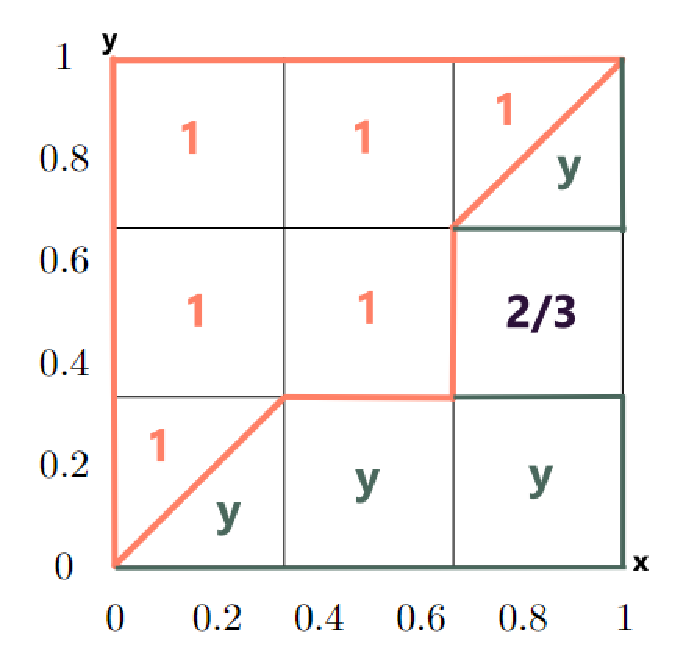
\includegraphics[scale=0.8]{template-fig/RPhi-impl.pdf}
    \end{graph}
\end{example}

Konstrukci tohoto reziduálního implikátoru lze popsat následovn\v e:\\
    Nech\v t  $\varphi:[0,1]\rightarrow [0,1]$ je funkce z příkladu \ref{sub: fi}.
Pak je reziduální implikace zalo\v zena na $C_\varphi$ dána p\v redpisem
$$ R_{C_\varphi}(x,y) = \begin{cases} 1, & \mbox{pokud } x\leq y \mbox{ nebo } (x,y) \in [\frac{1}{3},\frac{2}{3}]^2\\
\frac{2}{3}, &\mbox {pokud }
(x,y)\in [\frac{2}{3},1[\times[\frac{1}{3},\frac{2}{3}]
\\ y, &\mbox {jinak.}
\end{cases} $$

Pro obecnou neklesající a zleva spojitou funkci $\varphi$,  dostáváme fuzzy implikátor, kterého obecný předpis je v následujícím tvrzení.
\begin{sentence}
\cite{mitav}
\label{r-impl}
     Nechť je $\varphi:[0,1]\rightarrow [0,1]$
neklesající a zleva spojitá funkce na intervalu $]0,1[$.
Nechť je
$\{[a_i,b_i]\}_{i\in I}$ množina podintervalů intevalu $[0,1]$, přičemž $\varphi(x)=c_i$ pro $x\in
[a_i,b_i]$.
Potom je operátor $R_{C_\varphi}$ fuzzy implikací dán formulí

$$ R_{C_\varphi}(x,y) = \begin{cases} 1, & \mbox{pokud } x\leq y \mbox{ nebo } (x,y) \in [a_i,b_i]^2\\
1-\varphi^{(-1)}(c_i)=1-a_i, &\mbox {pokud }
(x,y)\in [b_i,1[\times[a_i,b_i]
\\ y, &\mbox {jinak.}
\end{cases} $$
\end{sentence}

Obecný průběh takového implikátoru pak lze vyjádřit následujícím grafem:
\begin{graph}
    Příklad obecného reziduálního implikátoru $R_{C_\varphi}$.
    \begin{figure}[H]
                \hspace{-1cm}
                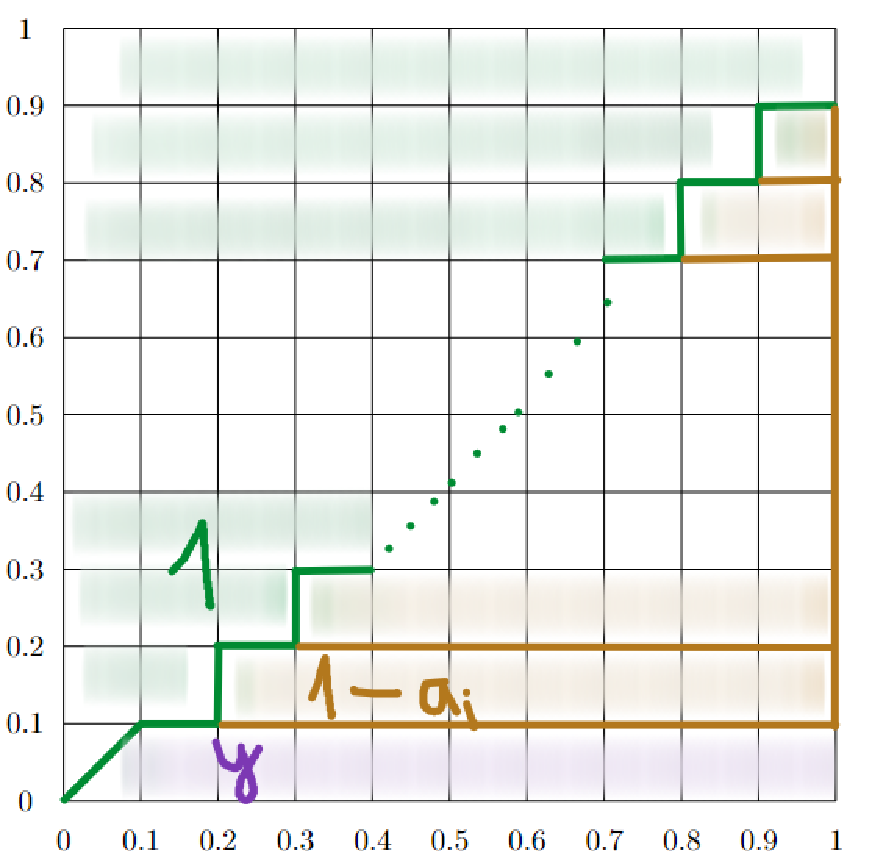
\includegraphics[scale=0.4]{template-fig/r-impliphi.pdf}
                \centering
            \end{figure}
\end{graph}


\subsubsection{Nová třída fuzzy implikací}
Pomocí výše popsané konstrukce získáváme další novou třídu fuzzy implikací. Na rozdíl od reziduálních implikací založených na zleva spojitých t-normách, tato nová třída nespl\v nuje vlastnost uspořádání. Také tuto konstrukci můžeme zobecnit a to použitím $\varphi-$transformace nějaké jiné t-normy.


\chapter{Modelování fuzzy logických spojek}
Tato kapitola popisuje využití dříve popsaných znalostí o fuzzy logických spojkách a jejich konstrukcí k tvorbě programu pro vyhodnocení pochopení implikací v běžném jazyce. Snažila jsem se tedy najít nejvhodnější algoritmus pro modelování (S,N)-implikací za pomocí triangulárních konorem a klasického negátoru. Využila jsem některé již známé algoritmy, které po jistých \' upravách vyhovují specifickým podmínkám plynoucích z vlastností t-norem. Celý sv\r uj program jsem postavila na již existujícím programu, jehož autorem je Ing. Vojtěch Havlena, Ph.D., který popisuje přesné znění jeho aplikace ve své bakalářské práci. \cite{havlena}

Pro modelování (S,N)-implikací je nejpodstatnější nalézt co nejvhodnější triangulární konormu, která co nejpřesněji odpovídá získaným empirickým dat\r um. Po \' upravě obecného principu aditivního generátoru spojité archimedovské t-normy \cite{alsina} lze na základě komplementarity funkcí získat předpis pro t-konormu takový, že $$S(x,y) = 1 - g^{(-1)}(g(1-x) + g(1-y)),$$ kde $g^{(-1)}$ je pseudoinverzní funkce k funkci g. Aproximace spojitých archimedovských t-norem poté po \' upravě pro t-konormy je vyjádřena následovně: $$S(x_1, x_2, \dots, x_n) = 1 - g^{-1}\left(\sum_{i = 1}^{n} g(1 - x_i)\right).$$
Aditivní generátor spojité archimedovské t-normy T je funkce klesající, při práci s t-konormami je funkce klesající, v dalších částech práce budeme pracovat s funkcí neklesající. Je tedy snadnější aproximovat samotné generátory, namísto norem a konorem. Níže popisuji takový postup.

\section{Aproximace aditivních generátor\r u}
Aditivní generátor výše popsaný lze aproximovat r\r uznými zp\r usoby. V našem případě využijeme tzv. spline křivky, konkrétně pak B-spline křivku. Aproximovaný aditivní generátor po drobné \' upravě vypadá následovně: $$g(1-u) = S_{k,x}(1-u) = \sum_{i = 1}^{n-1}c_iB_{i,k}(1-u),$$ kde \textit{$c_i$} jsou ovládací body křivky, \textit{$B_{i,k}(1-u)$} jsou základní funkce B-spline řádu \textit{k} a \textit{n} je počet ovládacích bod\r u.

Základní funkce B-spline řádu \textit{k} jsou definovány rekurzivně pro t-konormy: \\
\begin{itemize}
    \item Pro k = 1:
\[
N_{i,1}(u-1) = 
\begin{cases}
    0 & \text{pokud} \quad u_i \leq u < u_{i+1} \\
    1 & \text{jinak}
\end{cases}
\]

 \item Pro k > 1:
\[
N_{i,k}(u-1) = \frac{u - x_i}{x_{i + k - 1} - x_i} \cdot N_{i, k - 1}(u-1)
+ \frac{x_{i + k} - u}{x_{i + k} - x_{i + 1}} \cdot N_{i + 1, k - 1}(u-1)
\]
\end{itemize}



V následující kapitole je popsán experiment, při kterém jsem se snažila vyhodnotit, jak lidé v běžném vágním jazyce vnímají implikace. Využívám k tomu znalosti popsané výše, především pak znalosti o konstrukci t-norem, t-konorem a implikátorů. V 
první části zjišťuji, zda-li lidé chápou implikace jako ekvivalence nebo nikoliv. V druhé fázi experimentu hledám nejvhodnější fuzzy implikace, které  nejlépe aproximují funkce ze získaných empirických dat pomocí dotazníku.



\section{Experiment modelování fuzzy implikace}
V rámci své bakalářské práce provádím experiment, který využívá znalostí z předchozích kapitol a zaměřuje se na zjištění toho, zda lidé v běžném jazyce chápou implikace obdobně, jako je popisuje fuzzy matematika nebo nikoliv. Snažila jsem se tedy najít implikace, které budou co nejvíce odpovídat získaným funkcím ze zpracovaných dat a vlastně celkově zkoumat, zda lidé nerozumí implikacím spíše jako výrok\r um sobě ekvivalentním.

Data, která využívám pro provádění experimentu jsem získala pomocí mnou vytvořené dotazníkové webové aplikaci\footnote{Dotazník je dostupný pod odkazem: \href{https://www.stud.fit.vutbr.cz/~xjirmu00/bp/}{Dotazník}}. Dotazovaní měli za \' ukol přiřadit k předem připraveným výrok\r um nějakou číselnou hodnotu v rozmezí 0-10, přičemž 0 znamenalo, že s výrokem v\r ubec nesouhlasí a 10, že s ním plně souhlasí. Výrok\r u je celkově dvacet, přičemž se dělí na pět skupin po čtyřech výrocích, kde jsou první dva výroky $A$ a $B$ prosté, a další dva jsou tvořené implikací $A \to B$ a $B \to A$.

Respondenty jsem pečlivě vybírala velmi rozmanitě, protože je zřejmé, že technicky založené osoby vnímají výrokovou logiku více matematicky než-li ostatní lidé. Zvolila jsem tedy rozsáhlou škálu osob a na dotazník odpovídali jak studenti z informatických fakult, tak pracující z r\r uzných obor\r u netýkajících se informačních technologií, ale i d\r uchodci a další.

Použité výroky v dotazníku vypadaly následovně:
\begin{enumerate}
       \item  \clqq Testy z matematiky bývají zpravidla těžké.\crqq  , 
       \item  \clqq Výsledky z testu z matematiky jsou obvykle špatné.\crqq  ,
       \item  \clqq Pokud je test z matematiky těžký, mám z něj špatný výsledek.\crqq  ,
       \item  \clqq Pokud mám z testu z matematiky špatný výsledek, test byl těžký.\crqq  ,
       \item  \clqq Chodím dříve spát.\crqq  ,
       \item  \clqq Nebývám příliš unavený.\crqq  ,
       \item  \clqq Když půjdu brzy spát, budu další den méně unavený.\crqq  ,
       \item  \clqq Jsem-li méně unavený, šel jsem předchozí noc dříve spát.\crqq  ,
       \item  \clqq Jízdné je drahé.\crqq  ,
       \item  \clqq Jízda hromadnou dopravou je pohodlná.\crqq  ,
       \item  \clqq Jestliže je jízdné drahé, cesta hromadnou dopravou je pak pohodlná.\crqq,
       \item  \clqq Jestliže je cesta hromadnou dopravou pohodlná, jízdné je drahé.\crqq  ,
       \item  \clqq Jsem poměrně vysoký.\crqq  ,
       \item  \clqq Nosím větší velikost bot.\crqq  ,
       \item  \clqq Jsem-li vysoký, nosím pak obvykle větší velikost bot.\crqq  ,
       \item  \clqq Pokud nosím větší velikost bot, jsem pak obvykle vysoký.\crqq  ,
       \item  \clqq Jsem starý.\crqq,
       \item  \clqq Mám hodně zkušeností.\crqq,
       \item  \clqq Pokud jsem starý, mám hodně zkušeností.\crqq,
       \item  \clqq Mám-li hodně zkušeností, jsem starý.\crqq 
\end{enumerate}

Nakonec bylo získáno 149 vyplněných a odeslaných dotazník\r u od respondent\r u. Dotazník pracuje s celými hodnotami 0-10, které jsem poté pro lepší práci s daty zobrazila na interval [0,1], se kterým pak v následujících částech experimentu pracuji.

\subsection{Experiment zjiš\v tování, zda lidé chápou implikace jako ekvivalence}
Implikace i ekvivalence jsou v běžném jazyce lidmi hojně využívány. Problém při využívání těchto logických spojek však nastává při převodu běžného jazyka do matematiky a naopak a v jejich obecném chápání lidmi. Lidské chápání logických spojek, především pak implikace, je velmi rozmanité a matematicky nepřesné. Mějme výrok: \textit{\clqq Pokud venku prší, zmoknu.\crqq } Takový výrok je zřejmě implikací. V běžném jazyce ale nastává problém takový, že tento výrok m\r uže být chápán jako ekvivalence, protože pokud někdo tvrdí, že zmokl, venku dozajista pršelo. Stává se tedy, že lidé zamě\v nují implikaci za ekvivalenci, protože klasické porozumění implikace přesně neodpovídá její matematické definici.


Z matematiky tedy víme, že tabulka pravdivostních hodnot pro implikace složených z jednoduchých výrok\r u \textit{P} a \textit{Q} vypadá následovně:
\begin{table}[H]
    \centering
    \begin{tabular}{|c|c|c|}
        \hline
        \(P\) & \(Q\) & \(P \Rightarrow Q\) \\ 
        \hline
        0 & 0 & 1 \\ 
        \hline
        0 & 1 & 1 \\ 
        \hline
        1 & 0 & 0 \\ 
        \hline
        1 & 1 & 1 \\ 
        \hline
    \end{tabular}
    \caption{Pravdivostní hodnoty implikace (P $\Rightarrow$ Q)}
\end{table}

Největším problémem při výuce výrokové logiky, konkrétně v chápání implikace, je v lidském chápání prvních dvou řádk\r u. Pokud totiž není daný předpoklad splněný, výrok je pravdivý vždy, ale v běžném jazyce tak vnímaný není. V rámci tohoto experimentu se snažím zjistit, zda lidé chápou implikované výroky stejně jako ekvivalence, a proto logicky usuzují, že nesplnění předpokladu se běžně automaticky bere jako nepravdivý výrok.

Z dat získaných pomocí dotazníku popsaného výše filtruji pomocí Python skriptu hodnoty získaných z výsledku provedením implikace $A \to B$ a poté $B \to A$ v každé skupině výrok\r u. Takové hodnoty jsou po převodu diskrétní a na intervalu [0,1]. Hodnoty těchto složených výrok\r u následně porovnávám a pokud se výsledné hodnoty liší o maxim\' aln\v e 0.1, respektive o maxim\' aln\v e 0.2, respondent nahlíží na výroky jako na ekvivalence a nespatřuje tedy ve výroku implikaci. Takový proces jsem použila pro každou skupinu výrok\r u a výsledky na závěr porovnala. Výsledky zobrazuji pomocí koláčových graf\r u pro zvýšení přehlednosti, kde modrá barva zastává odlišné hodnoty výsledk\r u a oranžová hodnoty stejné (nebo velmi blízké), tedy ekvivalenci. Pokud tedy respondent označil výroky $A \to B$ a $B \to A$ stejnou nebo velmi podobnou hodnotou pravdivosti, znamenalo to, že vnímá výroky obdobně, a tedy v grafu spadá do části vybarvené oranžovou barvou a naopak.

\subsubsection{Skupina výrok\r u 1}
Jako první zkoumám výroky \textit{\clqq Pokud je test z matematiky těžký, mám z něj špatný výsledek,\crqq } \space a \textit{\clqq Pokud mám z testu z matematiky špatný výsledek, test byl těžký.\crqq } \space V tomto konkrétním případě se jednalo o velice těsné výsledky. Naprosto shodné nebo opravdu velmi podobné odpovědi mělo téměř $44 $\space$ \%$ respondent\r u a blízké hodnoty $58.8 $\space$ \%.$

\begin{graph}
Koláčové grafy reprezentující shodu v první skupině výrok\r u s odchylkou 0.1, respektive 0.2.
    \begin{figure}[H]
                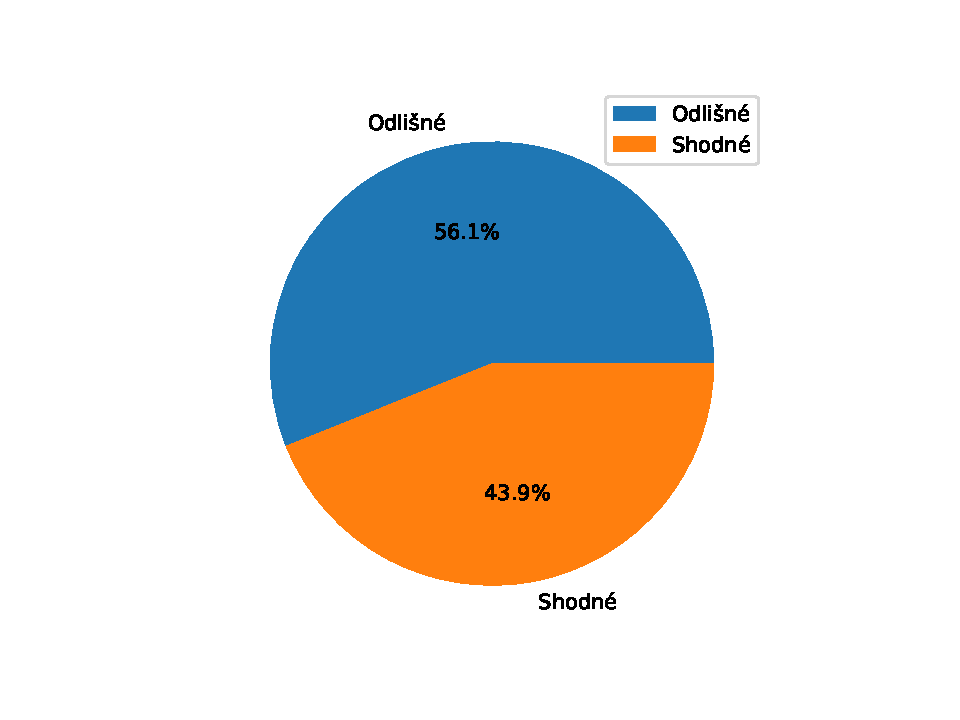
\includegraphics[scale=0.5]{template-fig/group0.pdf}
                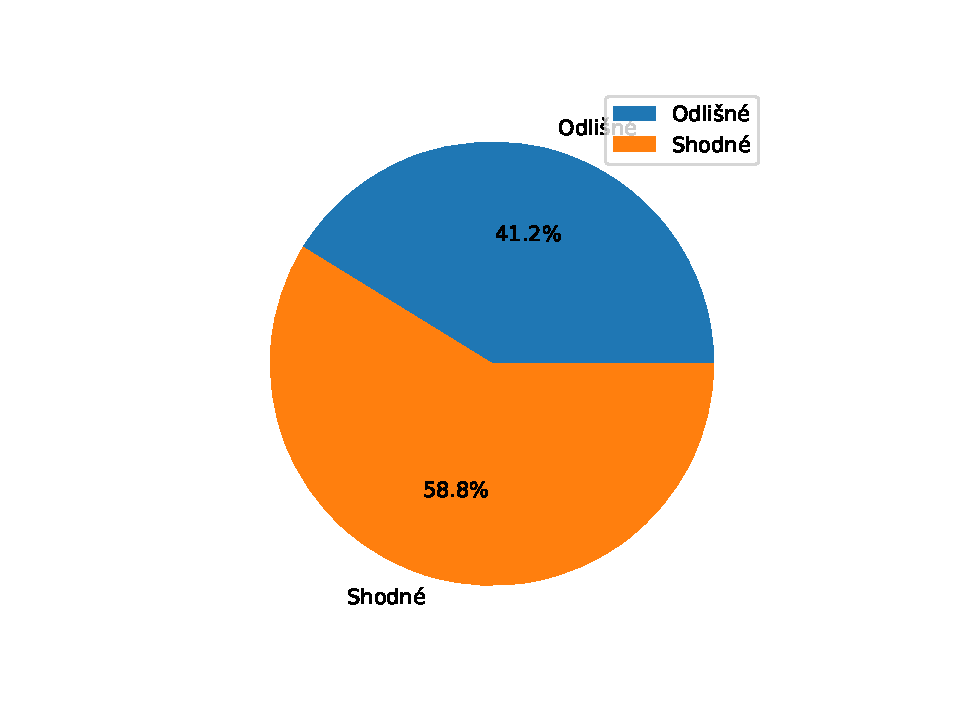
\includegraphics[scale=0.5]{template-fig/group00.pdf}
            \end{figure}
\end{graph}

\subsubsection{Skupina výrok\r u 2}
Další skupina výrok\r u sestává z vět \textit{\clqq Když půjdu brzy spát, budu další den méně unavený,\crqq } \space a \textit{\clqq Jsem-li méně unavený, šel jsem předchozí noc dříve spát.\crqq } \space  $50.7$ \space $\%$ respondent\r u vnímá výroky jako ekvivalenci. Většina lidí tedy vnímá vztah mezi \' unavou a spánkem rovnocenně a nezáleží jim na rozdílu vstupních předpoklad\r u, pravděpodoBně z toho d\r uvodu, že obecně je jízda hromadnou dopravou brána jako méně pohodlná varianta přepravy, ale i jako varianta levnější. Proto lidé mohou vnímat výroky jakožto ekvivalenci.
\begin{graph}
Koláčové grafy reprezentující shodu v druhé skupině výrok\r u s odchylkou 0.1, respektive 0.2.
    \begin{figure}[H]
                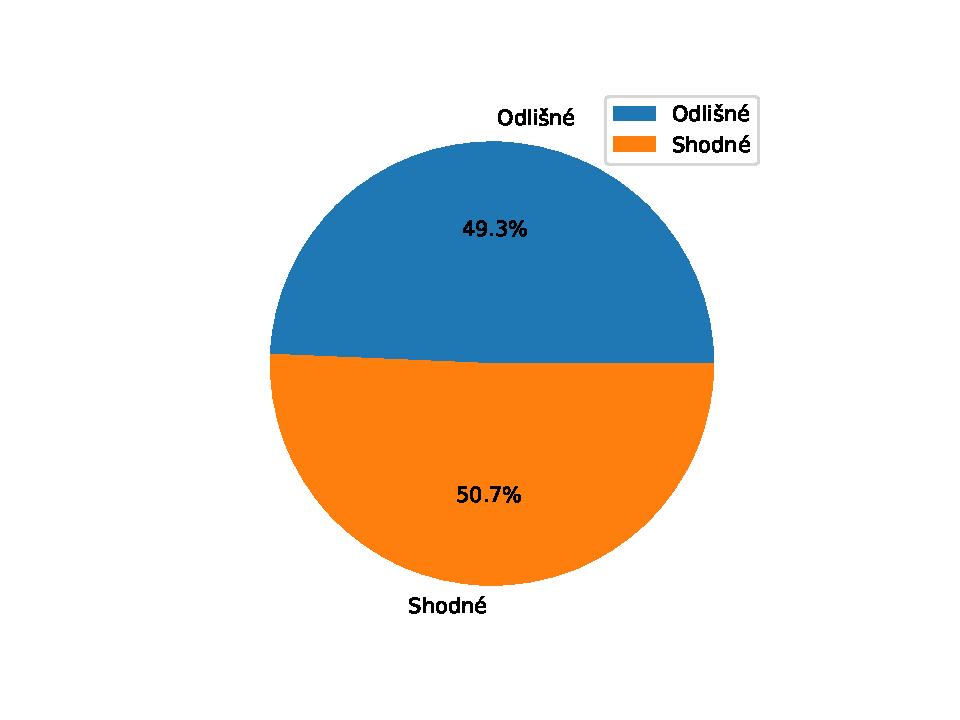
\includegraphics[scale=0.5]{template-fig/group1.pdf}
                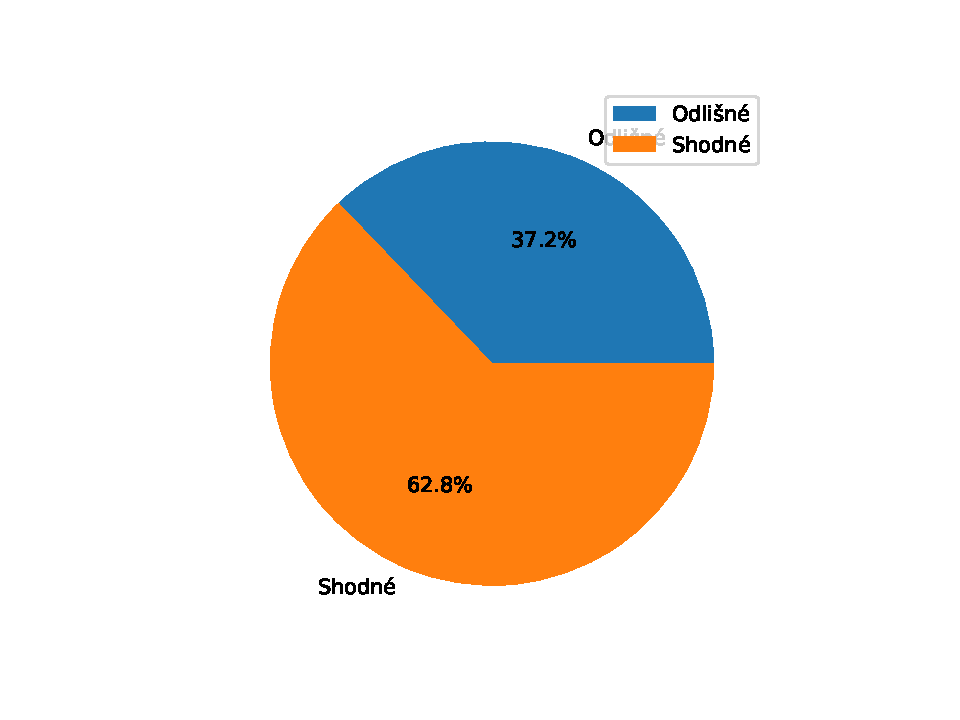
\includegraphics[scale=0.5]{template-fig/group11.pdf}
            \end{figure}
\end{graph}
\subsubsection{Skupina výrok\r u 3}
Pro výroky \textit{\clqq Jestliže je jízdné drahé, cesta hromadnou dopravou je pak pohodlná,\crqq } \space a \textit{\clqq Jestliže je cesta hromadnou dopravou pohodlná, jízdné je drahé,\crqq } \space m\r užeme pozorovat poměrně velkou převahu ekvivalentních odpovědí. Přes $60 $\space$ \%$ respondent\r u vyhodnotilo výroky rovnocenně a lidé ve většině nespatřovali ve větách implikaci.
\begin{graph}
Koláčové grafy reprezentující shodu ve třetí skupině výrok\r u s odchylkou 0.1, respektive 0.2.
    \begin{figure}[H]
                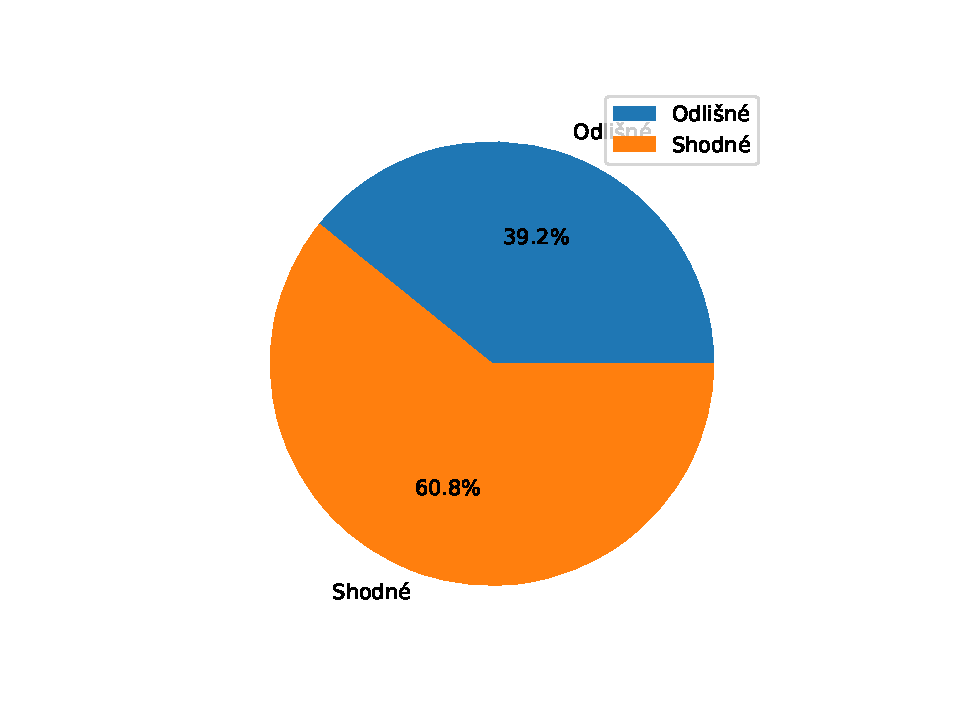
\includegraphics[scale=0.5]{template-fig/group2.pdf}
                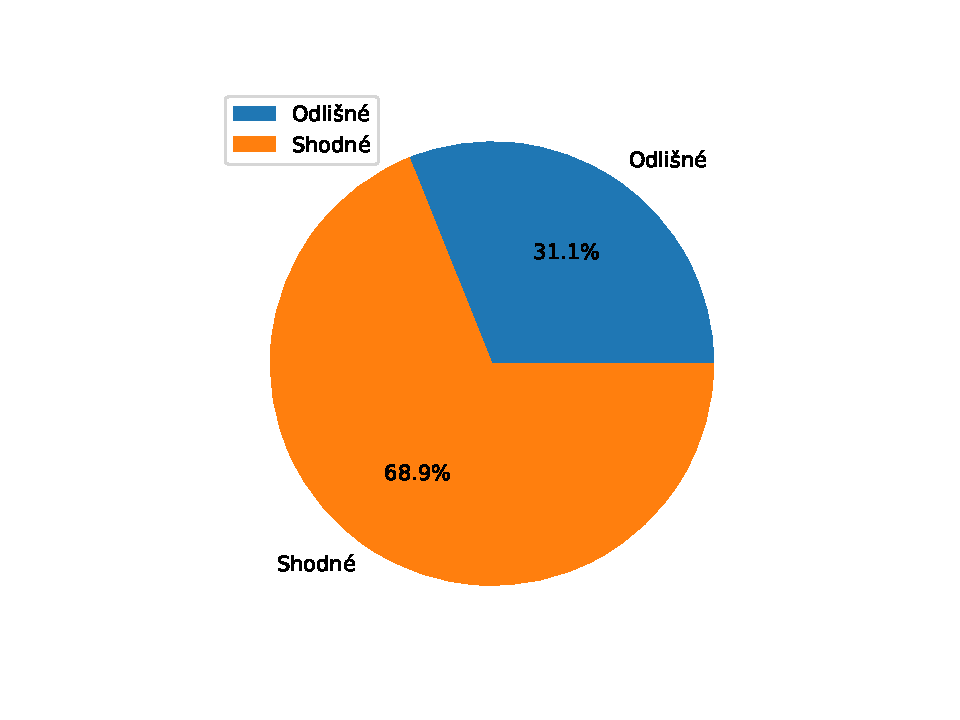
\includegraphics[scale=0.5]{template-fig/group22.pdf}
            \end{figure}
\end{graph}
\subsubsection{Skupina výrok\r u 4}
V této skupině výrok\r u m\r užeme pozorovat odpovědi, které se nejsilněji přibližují k logice ekvivalence. Jedná se o věty \textit{\clqq Jsem-li vysoký, nosím pak obvykle větší velikost bot,\crqq } \space a \textit{\clqq Pokud nosím větší velikost bot, jsem pak obvykle vysoký.\crqq } \space Výsledky s odchylkou 2 stup\v n\r u osy říkají, že $74,3 $\space$ \%$ respondent\r u vnímá výroky z obou stran stejně. Tato skupina výrok\r u je zadána velmi vágně, přičemž pojmy \textit{\clqq vysoký\crqq  a \clqq větší\crqq } jsou velmi nespecifické, a každý člověk je vnímá velmi rozdílně, proto mohou mít výroky v obecné řeči blíže k ekvivalenci.
\begin{graph}
Koláčové grafy reprezentující shodu ve čtvrté skupině výrok\r u s odchylkou 0.1, respektive 0.2.
    \begin{figure}[H]
                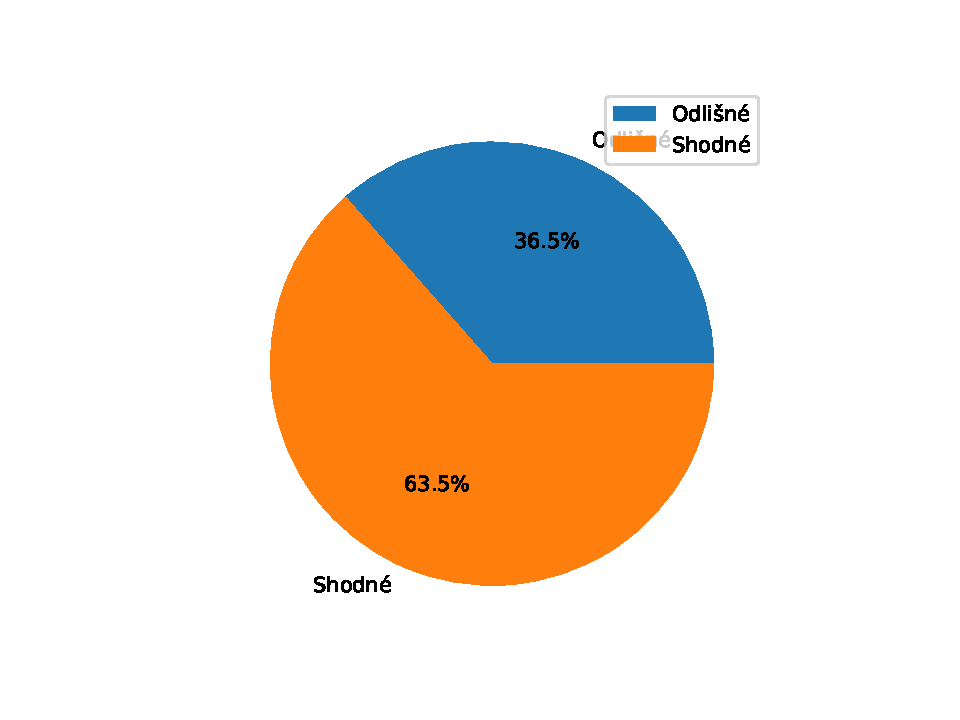
\includegraphics[scale=0.5]{template-fig/group3.pdf}
                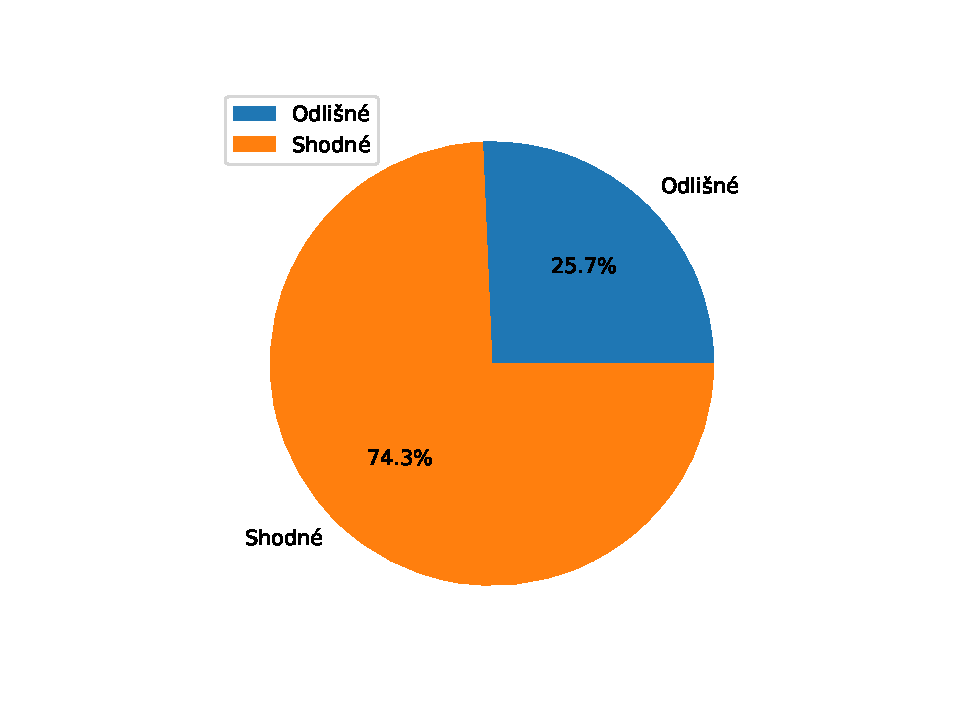
\includegraphics[scale=0.5]{template-fig/group33.pdf}
            \end{figure}
\end{graph}
\subsubsection{Skupina výrok\r u 5}
Na poslední skupinu výrok\r u bylo nahlíženo jako na výroky nejméně ekvivalentní. Jde o věty \textit{\clqq Pokud jsem starý, mám hodně zkušeností,\crqq }  \space a \textit{\clqq Mám-li hodně zkušeností, jsem starý.\crqq } \space Pouze $41.2 $\space$ \%$ respondent\r u vnímá věty jako sobě rovné. Výroky byly vytvořeny s menší mírou vágnosti a pojem \textit{\clqq starý\crqq } obecně lidé chápou poměrně striktně, na rozdíl od výroku \textit{\clqq hodně zkušeností. \crqq  \space} Z toho d\r uvodu lidé více dávají d\r uraz na předpoklad.
\begin{graph}
Koláčové grafy reprezentující shodu v páté skupině výrok\r u s odchylkou 0.1, respektive 0.2.
    \begin{figure}[H]
                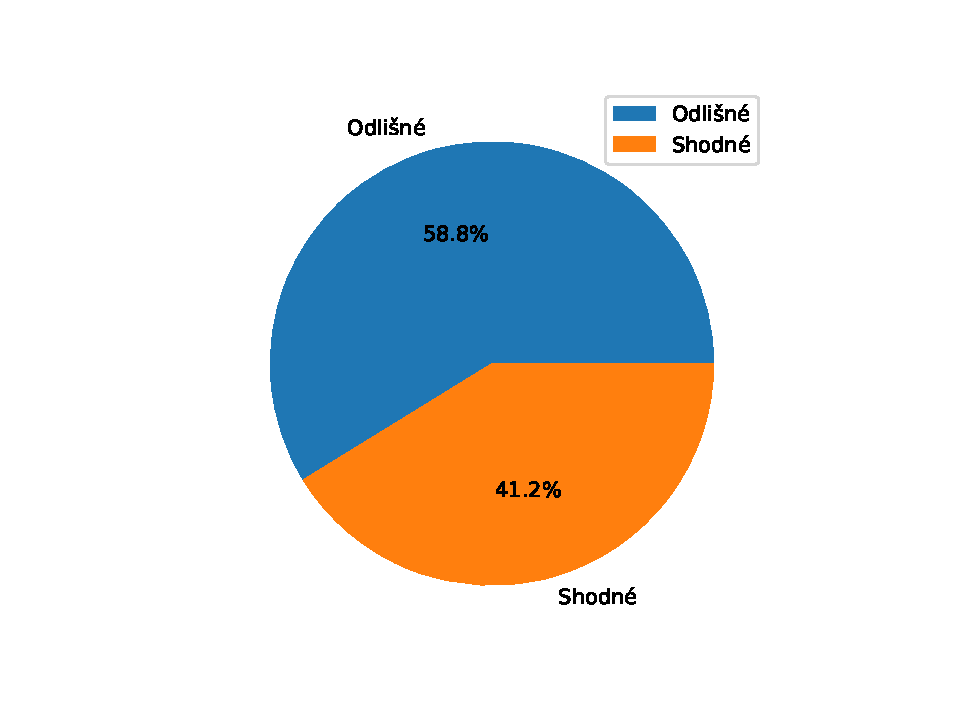
\includegraphics[scale=0.5]{template-fig/group4.pdf}
                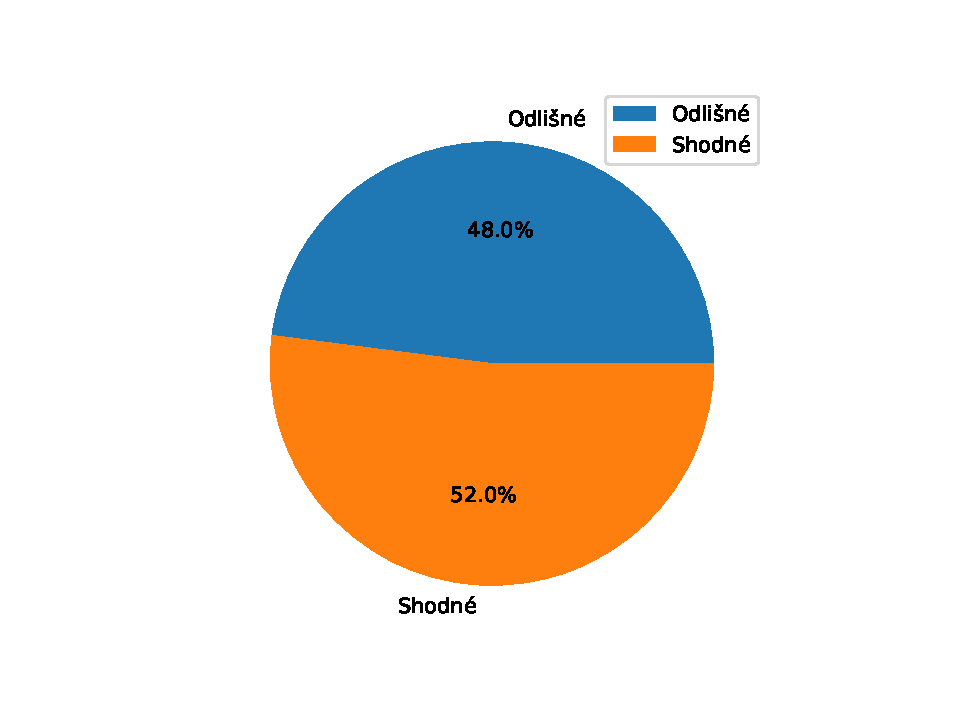
\includegraphics[scale=0.5]{template-fig/group44.pdf}
            \end{figure}
\end{graph}

Celkově tedy z experimentu vyplývá, že lidé nahlížejí na složené výroky pomocí implikace spíše jako na výroky ekvivalentní, což pak zp\r usobuje problémy při výuce výrokové logiky, kdy studenti přirozeně zamě\v nují implikace za ekvivalence, protože je tak lidé v běžném jazyce používají. Lidské vnímání jazyka je ale natolik vágní, že nelze označit všechny implikované výroky v běžné řeči za ekvivalence. V experimentu je ve skupině 5 ukázáno, že méně než polovina respondent\r u vnímala věty ekvivalentně, přičemž onen totožný vzorek lidí z velké části výroky 4 vnímal rovnocenně. Každá skupina výrok\r u je zadána s jinou mírou vágnosti, což se na výsledcích také velmi projevilo.

\chapter{Závěr}